%% Copernicus Publications Manuscript Preparation Template for LaTeX Submissions
%% ---------------------------------
%% This template should be used for copernicus.cls
%% The class file and some style files are bundled in the Copernicus Latex Package, which can be downloaded from the different journal webpages.
%% For further assistance please contact Copernicus Publications at: production@copernicus.org
%% https://publications.copernicus.org/for_authors/manuscript_preparation.html


%% Please use the following documentclass and journal abbreviations for preprints and final revised papers.

%% 2-column papers and preprints
\documentclass[acp, manuscript]{copernicus}

%% Journal abbreviations (please use the same for preprints and final revised papers)


% Advances in Geosciences (adgeo)
% Advances in Radio Science (ars)
% Advances in Science and Research (asr)
% Advances in Statistical Climatology, Meteorology and Oceanography (ascmo)
% Annales Geophysicae (angeo)
% Archives Animal Breeding (aab)
% Atmospheric Chemistry and Physics (acp)
% Atmospheric Measurement Techniques (amt)
% Biogeosciences (bg)
% Climate of the Past (cp)
% DEUQUA Special Publications (deuquasp)
% Drinking Water Engineering and Science (dwes)
% Earth Surface Dynamics (esurf)
% Earth System Dynamics (esd)
% Earth System Science Data (essd)
% E&G Quaternary Science Journal (egqsj)
% EGUsphere (egusphere) | This is only for EGUsphere preprints submitted without relation to an EGU journal.
% European Journal of Mineralogy (ejm)
% Fossil Record (fr)
% Geochronology (gchron)
% Geographica Helvetica (gh)
% Geoscience Communication (gc)
% Geoscientific Instrumentation, Methods and Data Systems (gi)
% Geoscientific Model Development (gmd)
% History of Geo- and Space Sciences (hgss)
% Hydrology and Earth System Sciences (hess)
% Journal of Bone and Joint Infection (jbji)
% Journal of Micropalaeontology (jm)
% Journal of Sensors and Sensor Systems (jsss)
% Magnetic Resonance (mr)
% Mechanical Sciences (ms)
% Natural Hazards and Earth System Sciences (nhess)
% Nonlinear Processes in Geophysics (npg)
% Ocean Science (os)
% Polarforschung - Journal of the German Society for Polar Research (polf)
% Primate Biology (pb)
% Proceedings of the International Association of Hydrological Sciences (piahs)
% Safety of Nuclear Waste Disposal (sand)
% Scientific Drilling (sd)
% SOIL (soil)
% Solid Earth (se)
% The Cryosphere (tc)
% Weather and Climate Dynamics (wcd)
% Web Ecology (we)
% Wind Energy Science (wes)


%% \usepackage commands included in the copernicus.cls:
%\usepackage[german, english]{babel}
%\usepackage{tabularx}
%\usepackage{cancel}
%\usepackage{multirow}
%\usepackage{supertabular}
%\usepackage{algorithmic}
%\usepackage{algorithm}
%\usepackage{amsthm}
%\usepackage{float}
%\usepackage{subfig}
%\usepackage{rotating}

\usepackage[acronym]{glossaries}
% \makeglossaries
\newacronym{abi}{ABI}{Advanced Baseline Imager}
\newacronym{amv}{AMV}{Atmospheric Motion Vector}
\newacronym{boa}{BoA}{Bottom-of-Atmosphere}
\newacronym{bt}{BT}{Brightness Temperature}
\newacronym{cape}{CAPE}{Convective Available Potential Energy}
\newacronym{cc4cl}{CC4CL}{Community Cloud Retrieval for Climate}
\newacronym{cci}{CCI}{Climate Change Initiative}
\newacronym{ccn}{CCN}{Cloud Condensation Nuclei}
\newacronym{ceres}{CERES}{Clouds and the Earth's Radiant Energy System}
\newacronym{cin}{CIN}{Convective Inhibition}
\newacronym{conus}{CONUS}{Continental United States}
\newacronym{cpr}{CPR}{Cloud Profiling Radar}
\newacronym{cre}{CRE}{Cloud Radiative Effect}
\newacronym{cth}{CTH}{Cloud Top Height}
\newacronym{ctt}{CTT}{Cloud Top Temperature}
\newacronym{cb}{Cb}{Cumulonimbus}
\newacronym[% options to override defaults
    shortplural={DCCs},
    longplural={Deep Convective Clouds}
    ]{dcc}{DCC}{Deep Convective Cloud}
\newacronym{dis}{DIS}{Deep Inverse Search}
\newacronym{dualtvl1}{Dual TV-L\textsuperscript{1}}{Dual Total Variation Regularisation \& Robust L\textsuperscript{1} Norm}
\newacronym{ebaf}{EBAF}{Energy Balanced and Filled}
\newacronym{esa}{ESA}{European Space Agency}
\newacronym{eumetsat}{EUMETSAT}{European Organisation for the Exploitation of Meteorological Satellites}
\newacronym{far}{FAR}{False Alarm Rate}
\newacronym{fat}{FAT}{Fixed Anvil Temperature}
\newacronym{gcm}{GCM}{Global Climate Model}
\newacronym{ghg}{GHG}{Greenhouse Gas}
\newacronym{glm}{GLM}{Geostationary Lightning Mapper}
\newacronym{goes}{GOES}{Geostationary Operational Environment Satellite}
\newacronym{inp}{INP}{Ice Nucleating Particle}
\newacronym{ir}{IR}{Infrared}
\newacronym{itcz}{ITCZ}{Inter-Tropical Convergence Zone}
\newacronym{jaxa}{JAXA}{Japan Aerospace Exploration Agency}
\newacronym{jma}{JMA}{Japanese Meteorological Agency}
\newacronym{lcl}{LCL}{Lifted Condensation Level}
\newacronym{lfc}{LFC}{Level of Free Convection}
\newacronym{lnb}{LNB}{Level of Neutral Buoyancy}
\newacronym{lw}{LW}{Longwave}
\newacronym{lwc}{LWC}{Liquid Water Content}
\newacronym{mcmip}{MCMIP}{Multi-channel Cloud and Moisture Imagery Product}
\newacronym{mcs}{MCS}{Mesoscale Convective System}
\newacronym{mse}{MSE}{Mean Square Error}
\newacronym{msg}{MSG}{Meteosat Second Generation}
\newacronym{nexrad}{NEXRAD}{Next Generation (Weather) Radar}
\newacronym{ngp}{NGP}{Northern Great Plains}
\newacronym{nir}{NIR}{Near Infrared}
\newacronym{noaa}{NOAA}{National Oceanic and Atmospheric Administration}
\newacronym{od}{OD}{Optical Depth}
\newacronym{pbl}{PBL}{Planetary Boundary Layer}
\newacronym{pca}{PCA}{Principle Component Analysis}
\newacronym{phat}{PHAT}{Proportionately Higher Anvil Temperature}
\newacronym{pod}{POD}{Probability of Detection}
\newacronym{rgb}{RGB}{Red, Green, Blue}
\newacronym{re}{r\textsubscript{e}}{Effective Radius}
\newacronym{seviri}{SEVIRI}{Spinning Enhanced Visible Infra-Red Imager}
\newacronym{sw}{SW}{Shortwave}
\newacronym{swd}{SWD}{Split Window Difference}
\newacronym{toa}{ToA}{Top-of-Atmosphere}
\newacronym{usa}{USA}{United States of America}
\newacronym{utc}{UTC}{Universal Co-ordinated Time}
\newacronym{wsr88d}{WSR-88D}{Weather Surveillance Radar, 1988, Doppler}
\newacronym{wv}{WV}{Water Vapour}
\newacronym{wvd}{WVD}{Water Vapour Difference}

\begin{document}

\title{A Lagrangian Perspective on the Lifecycle and Cloud Radiative Effect of Deep Convective Clouds Over Africa}

% \Author[affil]{given_name}{surname}
\Author[1]{William K.}{Jones}
\Author[2]{Martin}{Stengel}
\Author[1]{Philip}{Stier}

\affil[1]{Atmospheric, Oceanic and Planetary Physics, Department of Physics, University of Oxford}
\affil[2]{Deutscher Wetterdienst (DWD)}

%% The [] brackets identify the author with the corresponding affiliation. 1, 2, 3, etc. should be inserted.

%% If an author is deceased, please mark the respective author name(s) with a dagger, e.g. "\Author[2,$\dag$]{Anton}{Smith}", and add a further "\affil[$\dag$]{deceased, 1 July 2019}".

%% If authors contributed equally, please mark the respective author names with an asterisk, e.g. "\Author[2,*]{Anton}{Smith}" and "\Author[3,*]{Bradley}{Miller}" and add a further affiliation: "\affil[*]{These authors contributed equally to this work.}".


\correspondence{William K. Jones (william.jones@physics.ox.ac.uk)}

\runningtitle{A Lagrangian Perspective on the Lifecycle and Cloud Radiative Effect of Deep Convective Clouds Over Africa}

\runningauthor{William K. Jones et al.}

\received{}
\pubdiscuss{} %% only important for two-stage journals
\revised{}
\accepted{}
\published{}

%% These dates will be inserted by Copernicus Publications during the typesetting process.

\firstpage{1}

\maketitle



\begin{abstract}
The anvil clouds of tropical deep convection have large radiative effects in both the shortwave (SW) and longwave (LW) spectra with the average magnitudes of both over 100\,\unit{Wm\textsuperscript{-2}}. Despite this, due to the opposite sign of these fluxes, the net average of anvil cloud radiative effect (CRE) over the tropics is observed to be neutral. Research into the response of anvil CRE to climate change has primarily focused on the feedbacks of anvil cloud height and anvil cloud area, in particular regarding the LW feedback. However, tropical deep convection over land has a strong diurnal cycle which may couple with the shortwave component of anvil cloud radiative effect. As this diurnal cycle is poorly represented in climate models it is vital to gain a better understanding of how its changes impact anvil CRE.

To study the connection between deep convective cloud (DCC) lifecycle and CRE, we investigate the behaviour of both isolated and organised DCCs in a 4-month case study over sub-Saharan Africa (May-August 2016). Using a novel cloud tracking algorithm, we detect and track growing convective cores and their associated anvil clouds using geostationary satellite observations from Meteosat SEVIRI. Retrieved cloud properties and derived broadband radiative fluxes are provided by the CC4CL algorithm. By collecting the cloud properties of the tracked DCCs, we produce a dataset of anvil cloud properties along their lifetimes. While the majority of DCCs tracked in this dataset are isolated, with only a single core, the overall coverage of anvil clouds is dominated by those of clustered, multi-core anvils due to their larger areas and lifetimes.

We find that the anvil cloud CRE of our tracked DCCs have a bimodal distribution. The interaction between the lifecycles of DCCs and the diurnal cycle of insolation results in a wide range of SW anvil CRE, while the LW component remains in a comparatively narrow range of values. The CRE of individual anvil clouds varies widely, with isolated DCCs tending to have large negative or positive CREs while larger, organised systems tend to have CRE closer to zero.  Despite this, we find that the net anvil cloud CRE across all tracked DCCs is close to neutral (--0.94\,\textpm\,0.91\,\unit{Wm\textsuperscript{-2}}). Changes in the lifecycle of DCCs, such as shifts in the time of triggering, or the length of the dissipating phase, could have large impacts on the SW anvil CRE and lead to complex responses that are not considered by theories of LW anvil CRE feedbacks.

\end{abstract}


\copyrightstatement{TEXT} %% This section is optional and can be used for copyright transfers.


\introduction  %% \introduction[modified heading if necessary]

\acrfullpl{dcc} play a key role in the tropical atmosphere. 
Forming the ascending branch of the Hadley cells near the equator, \acrshort{dcc}s are critical to the circulation and heat transfer of the tropics \citep{riehl_heat_1958, weisman_mesoscale_2015}. 
\acrshort{dcc}s are also a cause of extreme weather events including floods, lightning and hail \citep{westra_future_2014}. 
\acrfullpl{mcs}---large, long-lived convective systems in which the anvils of multiple convective cores combine into a single, large `cloud shield' \citep{chen_diurnal_1997, houze_mesoscale_2004, roca_simple_2017}---are responsible for the majority of precipitation in the tropics \citep{feng_global_2021}. 
Changes in the behaviour of \acrshort{dcc}s with climate change have the potential for major impacts on the atmosphere, weather and society.

\acrshort{dcc}s also exert a key influence on the temperature of the tropics through their \acrfull{cre}. 
Due to their size, height and depth, \acrshort{dcc} anvils have large radiative effects in both the \acrfull{sw} and \acrfull{lw}, with both having average magnitudes exceeding 100\,\unit{W m^{-2}} \citep{hartmann_tropical_2016, wall_balanced_2018}. 
However, due to the opposite signs of these two components, the average anvil \acrshort{cre} in the tropics is approximately zero \citep{ramanathan_cloudradiative_1989, hartmann_effect_1992, stephens_cloudsat_2018}. 
Radiation is also key to the lifecycle of \acrshort{dcc}s. 
Over land, convection is typically initiated by the heating of the surface and lower troposphere by solar \acrshort{sw} radiation, resulting in a peak of convective activity in the late afternoon. 
Over the ocean, however, convection is often triggered by \acrshort{lw} cooling of the upper troposphere, and so convective activity occurs more frequently in the morning. 
However, the occurrence of convection is more uniform throughout the diurnal cycle compared to that over land \citep{taylor_evaluating_2017}. 
Radiation also has an impact on \acrshort{dcc} lifecycle through the differential heating of the anvil cloud, which destabilises the anvil cloud leading to dissipation due to entrainment and evaporation. 
However, \acrshort{sw} heating of the anvil cloud top during daytime acts to stabilise and delay this process, leading to differences in anvil lifetime depending on the diurnal cycle \citep{harrop_role_2016, sokol_tropical_2020, wall_observational_2020}.

There are several hypotheses regarding the \acrshort{cre} of tropical anvil clouds that consider whether the neutral \acrshort{cre} of tropical anvils is the result of a feedback mechanism. 
\citet{ramanathan_cloudradiative_1989} proposed the thermostat hypothesis in which, in response to a warming environment, anvil clouds produce thicker cirrus which acts to cool the tropics through increased \acrshort{sw} reflectance. 
The Iris hypothesis proposes that anvil cirrus will decrease in area, resulting in greater \acrshort{lw} emission from the surrounding clear-sky regions.
\citet{lindzen_does_2001} first proposed this as a result of increased precipitation efficiency, however evidence for this effect is disputed \citep{delgenio_climatic_2002, lin_examination_2004}.
\citet{bony_thermodynamic_2016} proposed a `stability iris' feedback, in which the established trends of increased dry static stability \citep{held_robust_2006} and a reduction in the tropical overturning circulation \citep{vecchi_global_2007} reduce the detrainment of anvil cirrus.
Although the anvil cloud response is generally considered to have a negative climate feedback, the predicted magnitude varies widely, it represents the greatest uncertainty among all cloud feedbacks \citep{sherwood_assessment_2020}, and a positive feedback cannot be ruled out \citep{gasparini_opinion_2023b}.

On the other hand, the \acrfull{fat} hypothesis argues that the anvil \acrfull{ctt} remains constant in a warming climate, and the greater difference between anvil and surface temperature results in a positive \acrshort{lw} feedback \citep{hartmann_important_2002}.
The basis for \acrshort{fat} is that \acrshort{lw} cooling of the troposphere due to water vapour becomes inefficient below 220\,\unit{K} \citep{jeevanjee_simple_2020}, which, if relative humidity remains constant, fixes the top of the convectively active troposphere at this isotherm. 
While there is evidence that this is the case for the largest \acrshort{dcc} anvils, the increase in static stability may result in a reduced positive feedback due to a `proportionally higher' anvil temperature \citep{zelinka_why_2010} which more closely matches the \acrshort{lw} response of tropical clouds in global climate models.
While satellite observations have shown a trend in anvil cloud height \citep{norris_evidence_2016}, there is not yet sufficient evidence to distinguish this from inter-annual variability \citep{takahashi_when_2019}.
\citet{seeley_fat_2019}, argued that \acrshort{fat} is a weak constraint on anvil temperature as while the radiative tropopause temperature remains fixed, the temperature of the tropopause lapse rate inversion can vary widely. 
Furthermore, as anvils tend to detrain below the tropopause, \citep{takahashi_level_2017, wang_observational_2020}, anvil temperature and the tropopause temperature may only be weakly connected.
\citet{seidel_temperatures_2022} however found the inclusion of CO\textsubscript{2} radiative heating produces anvil temperatures consistent with \acrshort{fat}.

While the iris and \acrshort{fat} feedbacks may act to cancel each other out, and hence maintain the neutral \acrshort{cre} of tropical anvil clouds, other potential feedback mechanisms may influence this balance.
\citet{hill_climate_2023} showed recently that climate models underestimate dynamically driven cloud feedbacks.
Furthermore, convective instability is expected to scale with temperature in the same manner as the Clausius-Clapeyron relation \citep{seeley_why_2015, agard_clausius_2017}, and some observations of tropical anvil clouds have instead suggested that warming of the surface invigorates convection \citep{igel_cloudsat_2014}.
Multi-decadal satellite observations have shown a cooling of upper tropospheric cloud temperature over land \citep{liu_observed_2023}, indicating that changes in convective processes may lead to stronger cooling feedbacks.

Changes to the lifecycle and diurnal cycle of deep convection may also be an important factor, particularly when considering the \acrshort{sw} feedback. 
\citet{nowicki_observations_2004} used estimates of \acrfull{toa} \acrshort{lw} and \acrshort{sw} radiative fluxes from \acrfull{seviri} observations to estimate the diurnal cycle of anvil \acrshort{cre} over equatorial Africa and the equatorial Atlantic. 
They found that shifting the diurnal cycle of deep convection in these regions could change the \acrshort{cre} by \textpm 10\,\unit{Wm\textsuperscript{-2}}, but did not track the properties of individual \acrshort{dcc}s.
\citet{bouniol_macrophysical_2016} compared \acrshort{cre} and cloud radiative heating rates to anvil cloud properties to investigate how radiative heating affects the anvil cloud evolution.
These observations were made with polar orbiting instruments however, and they highlighted the need for geostationary observations to characterise the evolution of individual anvil clouds.
Subsequent research used \acrshort{dcc} tracking methods to better characterise the lifecycle of observed anvil clouds \citep{bouniol_life_2021}, but as the radiative flux data was provided by polar-orbiting satellites the \acrshort{cre} could not be measured over the lifetime of the \acrshort{dcc}.

In this article, we use a novel cloud tracking methodology in conjunction with derived all-sky and clear-sky radiative fluxes to characterise the \acrshort{cre} over the lifecycles of individual anvil clouds. 
This methodology is applied to 4 months of data produced for the \acrshort{esa} Cloud-\acrshort{cci}+ project over sub-Saharan Africa. 
This dataset allows us to investigate both the \acrshort{cre} of individual \acrshort{dcc}s, as well as the net anvil \acrshort{cre} over the entire region. 
We find that the overall distribution of anvil \acrshort{cre} is determined by the relationship between \acrshort{dcc} lifecycle and the diurnal cycle of the \acrshort{sw} \acrshort{cre}, and discuss the implications of this for the response of \acrshort{dcc}s to a changing climate.



\section{Data}

For this case study, we used data from \acrshort{seviri} \citep{aminou_msg_2002} aboard the \acrlong{msg} Meteosat-11 satellite, which is in a geostationary orbit above the equator at 0\textdegree W. 
We use data from 4 months (May--August 2016) over sub-Saharan Africa (approximately 18\,\textdegree W--46\,\textdegree E, 31\,\textdegree S--15\,\textdegree N) at the full resolution of \acrshort{seviri} (3\,\unit{km} at nadir) as well as retrieved cloud properties and derived broadband fluxes produced by the \acrshort{esa} Cloud-\acrshort{cci}+ project.
\acrfull{bt} from \acrshort{seviri} is used by the tracking algorithm, and reflectances and \acrshort{bt} are used by the cloud retrieval.

\acrshort{seviri} is a visible and \acrlong{ir} radiometer with a nadir spatial resolution of 3\,\unit{km} and a temporal sampling time of 15 minutes for the full earth disc. 
\acrshort{seviri} has 12 channels across the visible, \acrfull{nir} and thermal-IR spectrum, with one being a high-resolution visible channel with a nadir resolution of 1\,\unit{km}. 
A brief overview of these channels, along with which are used for tracking \acrshort{dcc}s and the cloud properties retrieval, is provided in table~\ref{table:seviri_channels}.


\begin{table*}[tb]
\caption{\acrshort{seviri} channels and their use in the \acrshort{dcc} tracking algorithm and cloud properties retrieval.
}
\label{table:seviri_channels}
\begin{tabular}{lllcc}
\tophline
Channel & Wavelength (\unit{\mu m}) & Description & Tracking & Retrieval\tabularnewline
\middlehline
1 & 0.64 & Visible & & \checkmark\tabularnewline
2 & 0.81 & \acrshort{nir} & & \checkmark\tabularnewline
3 & 1.64 & \acrshort{nir} & & \checkmark\tabularnewline
4 & 3.92 & \acrshort{nir} Window & & \checkmark\tabularnewline
5 & 6.25 & Upper troposphere \acrfull{wv} & \checkmark & \checkmark\tabularnewline
6 & 7.35 & Lower troposphere \acrshort{wv} & \checkmark & \checkmark\tabularnewline
7 & 8.70 & Mid-IR window & &\tabularnewline
8 & 9.66 & Ozone & &\tabularnewline
9 & 10.8 & Clean \acrshort{lw} window & \checkmark & \checkmark\tabularnewline
10 & 12.0 & Dirty \acrshort{lw} window & \checkmark & \checkmark\tabularnewline
11 & 13.4 & CO\textsubscript{2} & & \checkmark\tabularnewline
12 & 0.6--0.9 & High-resolution visible & &\tabularnewline
\bottomhline
\end{tabular}
\belowtable{}
\end{table*}

%%% TWO-COLUMN TABLE
%
%%t
%\begin{table*}[t]
%\caption{TEXT}
%\begin{tabular}{column = lcr}
%\tophline
%
%\middlehline
%
%\bottomhline
%\end{tabular}
%\belowtable{} % Table Footnotes
%\end{table*}
%

An example of observations from \acrshort{seviri} is shown in fig.~\ref{fig:seviri_obs_example} for 15:00:00~\acrshort{utc} on 1\textsuperscript{st} June 2016. 
A visible composite (fig.~\ref{fig:seviri_obs_example}\,a) is constructed using the 1.64\,\unit{\mu m} and 0.81\,\unit{\mu m} near-infrared and 0.64\,\unit{\mu m} visible channels for the \acrfull{rgb} channels respectively. 
In this composite, ice clouds (which appear cyan) can be seen over central Africa and the southern Atlantic. fig.~\ref{fig:seviri_obs_example}\,b shows the 10.8\,\unit{\mu m} brightness temperature for the same scene, showing the coldest temperatures for the high ice clouds over central Africa. 
Two combinations of channels are used for the detection of anvil clouds. 
The \acrfull{wvd}, shown in fig.~\ref{fig:seviri_obs_example}\,c, consists of the 6.3\,\unit{\mu m} \acrshort{bt} minus the 7.4\,\unit{\mu m} \acrshort{bt}. 
In clear skies the \acrshort{wvd} is negative, with values around --\,20 to --\,15 K, due to the higher, and thus colder, emission height of the 6.3\,\unit{\mu m} channel. 
In high, thick clouds, however, the temperatures of the 6.3 and 7.4\,\unit{\mu m} channels converge and so the \acrshort{wvd} becomes closer to 0. 
In the cases of the highest clouds, the \acrshort{wvd} can become positive due to emission from stratospheric WV in the 6.3\,\unit{\mu m} channel. The \acrfull{swd}, shown in fig.~\ref{fig:seviri_obs_example}\,d, consists of the 10.8\,\unit{\mu m} \acrshort{bt} channel minus the 12.0\,\unit{\mu m} channel. 
While the \acrshort{swd} is sensitive to near-surface WV due to absorption in the 12.0\,\unit{\mu m} channel, it is also sensitive to thin ice clouds due to the difference in emissivity of ice particles between the two channels. 
While for thick clouds the \acrshort{swd} will be 0 K, for thin ice clouds the lower emission height of the 10.8\,\unit{\mu m} \acrshort{bt} channel results in a positive value of 5 K.
The 10.8\,\unit{\mu m} and 12.0\,\unit{\mu m} channels of \acrshort{seviri} have relatively wide wavebands and as such are less sensitive to the presence of thin ice clouds.
As a result, we found that the detection of thin anvil is unreliable using this technique with \acrshort{seviri}, and so is not considered within this article.


\begin{figure*}[tp]
    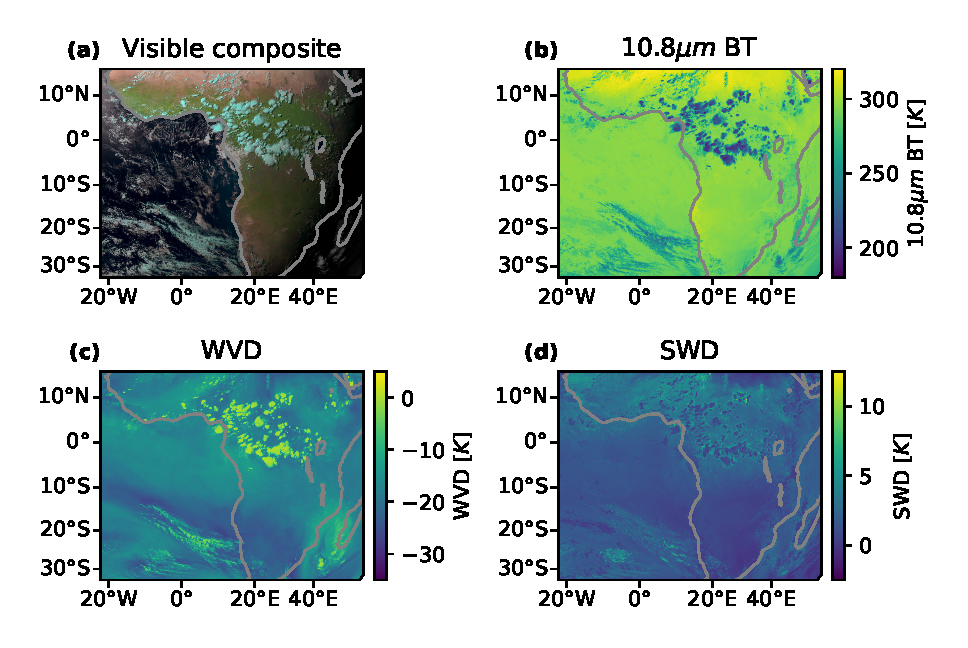
\includegraphics[width=12cm]{figures/fig01.pdf}
    \caption[
    Example observations from the Meteosat \acrshort{seviri} instrument at 15:00:00 \acrshort{utc} on 2016/6/01
    ]{
    Example observations from the Meteosat \acrshort{seviri} instrument at 15:00:00 \acrshort{utc} on 2016/6/01. a: A visible composite formed using the 1.6, 0.81 and 0.64\,\unit{\mu m} channels as the \acrshort{rgb} channels respectively, with 10.8\,\unit{\mu m} \acrshort{bt} during the night-time. The scene shows a cluster of cold cloud tops (cyan) over central Africa and over the Southern Atlantic. b: 10.8\,\unit{\mu m} \acrshort{bt}. c: \acrshort{wvd} formed by the 6.3\,\unit{\mu m} channel minus the 7.4\,\unit{\mu m} channel. d: \acrshort{swd} formed by the 10.8\,\unit{\mu m} channel minus the 12.0\,\unit{\mu m} channel.
    }
    \label{fig:seviri_obs_example}
\end{figure*}


Retrieved cloud properties, including optical thickness, effective radius, liquid/ice water path, \acrshort{ctt} and height, are provided by the \acrfull{cc4cl} algorithm \citep{sus_community_2018, mcgarragh_community_2018}. 
These properties are all retrieved at the same resolution as the input \acrshort{seviri} data. Broadband fluxes are derived using the BUGSRad radiative transfer model \citep{stephens_parameterization_2001} using input cloud properties from the \acrshort{cc4cl} retrieval and vertical temperature, moisture and trace gas profiles from ERA-5 \citep{hersbach_era5_2020}. 
The BUGSRad model provides \acrshort{toa} and \acrlong{boa} \acrshort{lw} and \acrshort{sw} radiative fluxes for both all-sky and clear-sky conditions. An example of these derived fluxes is shown in fig.~\ref{fig:seviri_flux_example}. 
Figure~\ref{fig:seviri_flux_example}\,a shows net \acrshort{toa} fluxes, with a net warming during the daytime on the Western side of the image, and a net cooling at night-time on the Eastern side. 
Figure~\ref{fig:seviri_flux_example}\,b shows the net \acrshort{toa} \acrshort{cre}, with a net cooling effect during the daytime and warming during the night-time for observed high clouds over central Africa. The \acrshort{sw} (fig.~\ref{fig:seviri_flux_example}\,c) and \acrshort{lw} (fig.~\ref{fig:seviri_flux_example}\,d) components of the \acrshort{cre} show that while the \acrshort{lw},
warming component has a smaller magnitude than the day-time, cooling \acrshort{sw} \acrshort{cre}, it remains constant during both day- and night-time.


\begin{figure*}[tp]
    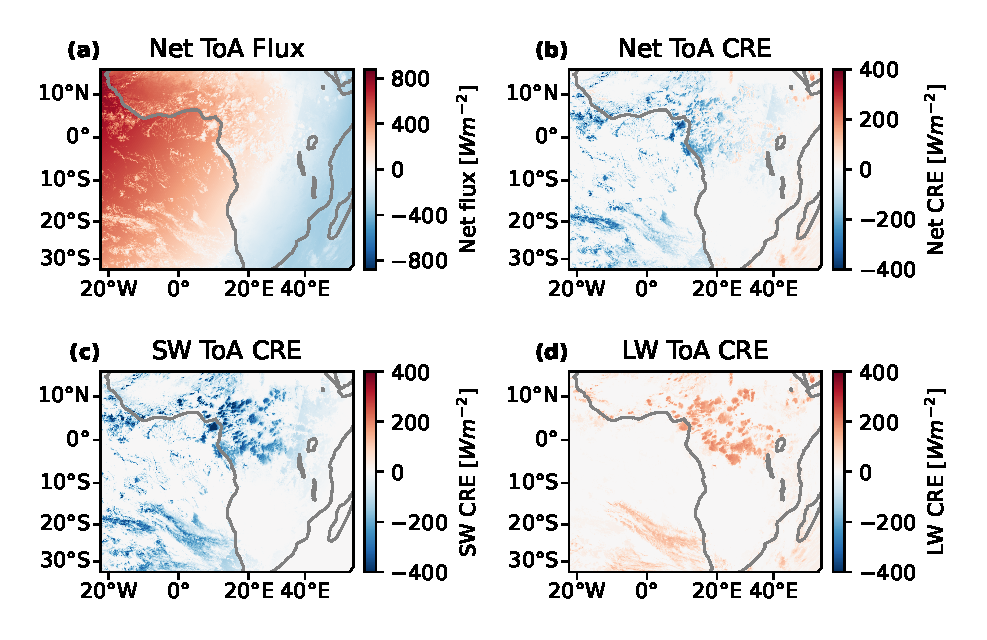
\includegraphics[width=12cm]{figures/fig02.pdf}
    \caption[
    An example of the \acrshort{toa} \acrshort{cre} derived using the radiative flux model
    ]{
    An example of the \acrshort{toa} \acrshort{cre} derived using the radiative flux model, for the same time
    as shown in fig.~\ref{fig:seviri_obs_example} (15:00:00 \acrshort{utc} on 2016/6/01). a: net \acrshort{toa} radiative flux. b: net \acrshort{toa} \acrshort{cre}. c: \acrshort{sw} downwards \acrshort{cre}. d: \acrshort{lw} downwards \acrshort{cre}.
    }
    \label{fig:seviri_flux_example}
\end{figure*}


Validation of the \acrshort{seviri} broadband fluxes was performed against monthly-mean observations of \acrshort{toa} broadband \acrshort{cre} from the \acrfull{ceres} \citep{loeb_clouds_2018} \acrfull{ebaf} climate data record. 
The results of this validation are shown in fig.~\ref{fig:flux_validation}. 
Monthly mean fluxes were calculated for \acrshort{seviri} by first calculating the mean daily fluxes over each 1\texttimes 1\textdegree grid square for days in which we have over 23 hours of observations, and then averaging these daily means over each month. 
Comparison of the net \acrshort{toa} \acrshort{cre} to \acrshort{ceres} revealed a bias of --\,1.87\,\unit{W m\textsuperscript{-2}} (fig.~\ref{fig:flux_validation}\,a,b), consisting of a \acrshort{sw} bias of --\,2.02\,\unit{W m^{-2}} (fig.~\ref{fig:flux_validation}\,c,d) and a \acrshort{lw} bias of +\,0.15\,\unit{W m\textsuperscript{-2}} (Fig~\ref{fig:flux_validation}\,e,f). 
Correction for these biases have been applied uniformly to all further \acrshort{cre} values given in this article.


\begin{figure*}[tp]
    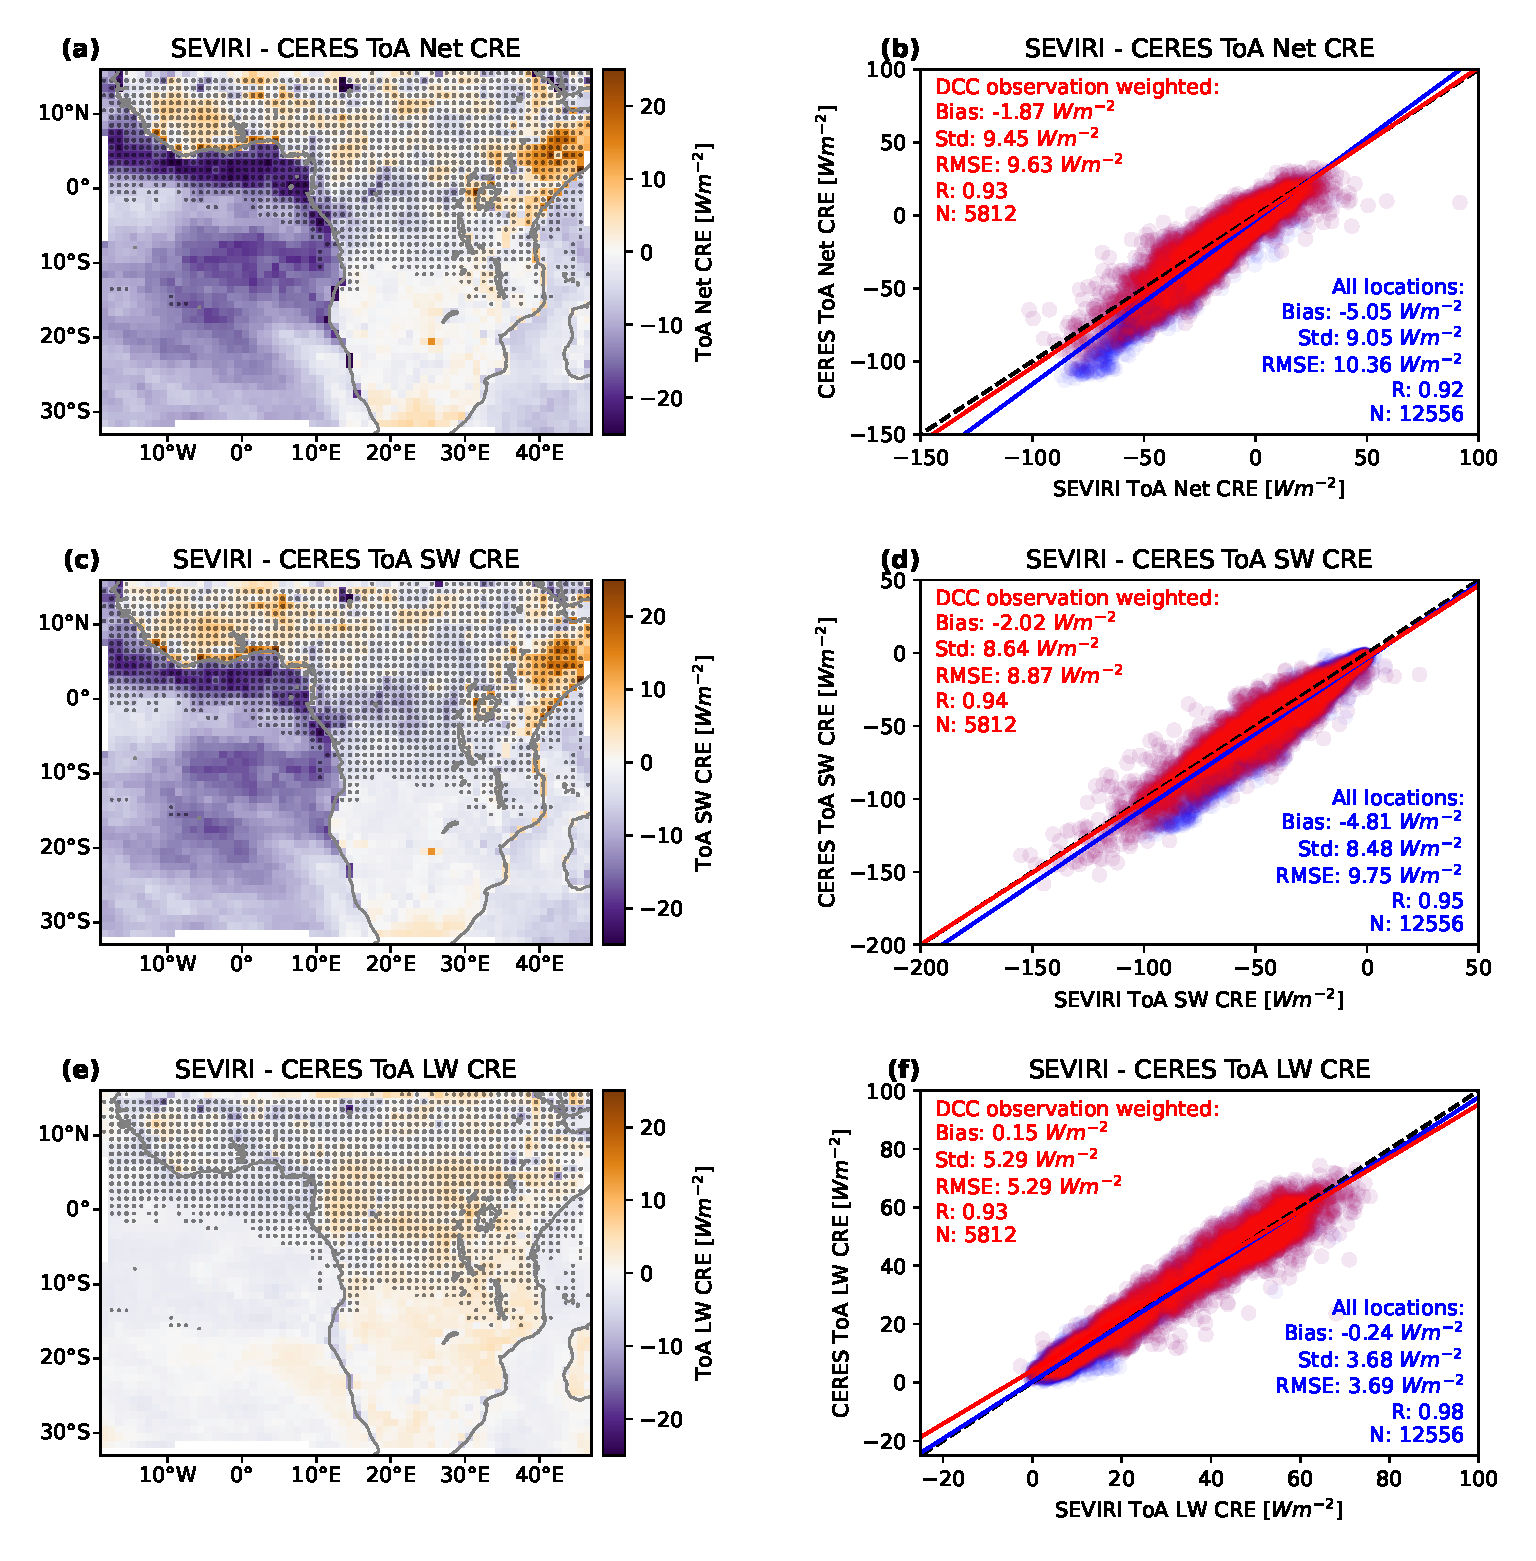
\includegraphics[width=12cm]{figures/fig03.pdf}
    \caption[
    Validation of derived broadband fluxes against monthly \acrshort{ceres}-\acrshort{ebaf} \acrshort{cre}
    ]{
    Validation of derived broadband fluxes against monthly \acrshort{ceres}-\acrshort{ebaf} \acrshort{cre}. a.: The mean difference in net \acrshort{toa} \acrshort{cre} by 1\texttimes 1\textdegree grid square. b.: A comparison of observed \acrshort{toa} net \acrshort{cre} for \acrshort{seviri} against \acrshort{ceres}, with all locations in blue, and those where we observe \acrshort{dcc} anvils in red. c.: the mean difference in \acrshort{sw} \acrshort{toa} \acrshort{cre}. d.: comparison of \acrshort{sw} \acrshort{toa} \acrshort{cre} for \acrshort{seviri} and \acrshort{ceres}. e.: the mean difference in \acrshort{lw} \acrshort{cre}. f.: comparison of \acrshort{lw} \acrshort{toa} \acrshort{cre}. The stippling in a, c and e represents the locations in which we observe \acrshort{dcc} anvils, with the size of the dots corresponding to the number of observations. The solid lines in b, d and f show the linear regression for all locations (blue) and the locations where we observe \acrshort{dcc} anvils (red) weighted by the number of observations.
    }
    \label{fig:flux_validation}
\end{figure*}

\section{Method}

The detection and tracking of \acrshort{dcc}s was performed using the tobac-flow algorithm \citep{jones_semilagrangian_2023}, which has been designed specifically to track both isolated and clustered \acrshort{dcc}s in geostationary satellite imagery over their entire lifecycle. 
While geostationary satellite imagery provides high-resolution observations over large domains and long time periods, which is ideal for studying deep convection, the inability of passive remote sensing to observe convective updrafts directly makes the detection and tracking of \acrshort{dcc}s difficult.

Algorithms for the detection and tracking of \acrshort{dcc}s in satellite imagery have generally been developed for one of two applications: tracking convective cores and isolated convection, or tracking large \acrshort{mcs} anvils.
Those designed for tracking deep convective cores, or isolated \acrshort{dcc}s, include Cb-TRAM \citep{zinner_cbtram_2008,zinner_validation_2013} or tobac \citep{heikenfeld_tobac_2019}.
These algorithms work by detecting regions of convective updraft or a proxy (such as cloud top cooling rate), and then treating these regions as point-like objects that are advected over time. 
The second group, designed for tracking \acrshort{mcs}s, include algorithms such as PyFLEXTRKR \citep{feng_pyflextrkr_2022}, TAMS \citep{nunezocasio_tracking_2020} or TOOCAN \citep{fiolleau_algorithm_2013}. 
These algorithms detect large regions of cold cloud tops which indicate anvil clouds, and then link them over time by overlapping regions at subsequent time steps. 
There is no `best' method for tracking all types of convection however \citep{lakshmanan_objective_2010}. 
The algorithms for tracking isolated convective cells perform worse for clustered convection when the motion and shape of the \acrshort{dcc} cannot be adequately represented as a single vector. 
On the other hand, the \acrshort{mcs} tracking algorithms perform worse for smaller, isolated \acrshort{dcc}s as the motion of the anvil between time steps may mean it does not overlap with the previous step.

To approach the challenge of tracking both isolated \acrshort{dcc}s and large, clustered systems, we address the role of cloud motion in the scaling problem. 
tobac-flow first estimates the motion of \acrshort{dcc}s at each pixel using an optical-flow algorithm. 
Then, using these estimated motion vectors, we construct a semi-Lagrangian framework in which to perform the detection and tracking. 
This approach addresses two issues found in traditional cloud tracking approaches.
First, estimating a motion vector for each pixel allows complex motions (including divergence, rotation, splitting and merging) to be compensated for, rather than just the bulk motion found using the centroid tracking methods.
Second, by estimating the cloud motion \textit{a priori}, we are able to use this information within the detection step of the algorithm, and can separate changes in cloud properties such as \acrshort{bt} from those observed due to cloud motion.
This framework removes the problem of \acrshort{dcc} motion, allowing us to track both isolated and large \acrshort{dcc}s at the same time.

Three channels and channel combinations from \acrshort{seviri} are used for the detection algorithm: the 10.8\,\unit{\mu m} \acrshort{bt} channel; the \acrshort{wvd} (the difference between the 6.2\,\unit{\mu m} and 7.3\,\unit{\mu m} channels), and the \acrshort{swd} (the difference between the 10.8\,\unit{\mu m} and 12.0\,\unit{\mu m} channels).
Estimation of cloud motion vectors using optical flow in performed using the 10.8\,\unit{\mu m} \acrshort{bt} channel.
Detection of cores utilises the 10.8\,\unit{\mu m} \acrshort{bt} channel and the \acrshort{wvd}, and detection of anvils uses \acrshort{wvd} and \acrshort{swd}.

We detect growing convective cores where we observe regions of rapid cooling in the 10.8\,\unit{\mu m} \acrshort{bt} channel of greater than 0.5\,\unit{Ks\textsuperscript{-1}} and the \acrshort{wvd} of greater than 0.25\,\unit{Ks\textsuperscript{-1}}.
In both cases
\acrshort{dcc}s close to the surface and continue tracking them into the upper troposphere. 
We classify a core as a region of cooling temperature that has existed for at least 15 minutes and has cooled by at least 8\,\unit{K} in a 15-minute period. 
This threshold provides a strong indicator of intense convective activity \citep{roberts_nowcasting_2003}, and so provides an accurate detection of growing \acrshort{dcc}s.

Starting from these convective cores, we then detect the surrounding anvil cloud using the \acrshort{wvd} field \citep{muller_role_2018, muller_novel_2019} and continue to detect the anvil until its dissipation, even after the core is no longer visible. 
A core and anvil are linked with each other if the two overlap at a time when the core has mean \acrshort{wvd} of \textgreater\,5\,\unit{K}, indicating that it has reached the upper troposphere.
Each anvil cloud can be associated with multiple cores, allowing us to identify cases of clustered convection. 
As we detect the cores based on cloud-top cooling, however, we can only detect the cores themselves during the growing phase, and cannot detect cores that occur underneath cold, high, anvil clouds.
When determining the number of cores associated with an anvil, we count the total number of cores observed over the entire lifetime, even if they do not occur at the same time, and including all merges and splits of the anvil cloud.
This flexibility allows for a wide range of different organised systems to be analysed.

Due to the lack of sensitivity of the \acrshort{seviri} \acrshort{swd} to thin ice clouds, we only detect and track the thick portion of the anvil in this article.
The \acrshort{wvd} channel of \acrshort{seviri} is capable of detecting anvils with optical thicknesses of approximately 1--1.5 (see supplementary fig. S1).
However, the closer spacing and narrower bandwidth of the \acrshort{seviri} \acrshort{lw} window channels (see supplementary fig. S2), along with the higher noise means that the \acrshort{swd} is less sensitive to thin cirrus compared to instruments such as the \acrshort{goes}-16 advanced baseline imager (see supplementary fig. S3).
The anvils tracked in this paper have a median retrieved minimum optical depth at 0.64\,\unit{\mu m} of 1.45, although this value is likely biased high as many anvils dissipate at night when accurate satellite retrievals of optical depth are not available.
While this sensitivity captures much of the \acrshort{cre} of \acrshort{dcc} anvils \citep{berry_cloud_2014} the long lifetimes of dissipating thin anvils may have a significant warming contribution to net anvil \acrshort{cre} \citep{horner_evolution_2023}.
As a result, it is expected that the anvil \acrshort{cre} measured in this study is biased low.

An example of the cores and anvils detected by the tobac-flow algorithm is shown in fig.~\ref{fig:seviri_detection}, at 3-hour intervals. In fig.~\ref{fig:seviri_detection}\,a, we see a large number of developing cores over central Africa. 
In fig.~\ref{fig:seviri_detection}\,b, we see more developing cores over Western Africa as the pattern of initiation has shifted with the diurnal cycle.
In fig.~\ref{fig:seviri_detection}\,c,d we observe fewer new developing cores later in the day, but the larger anvil clouds persist into the night-time.


\begin{figure*}[tp]
    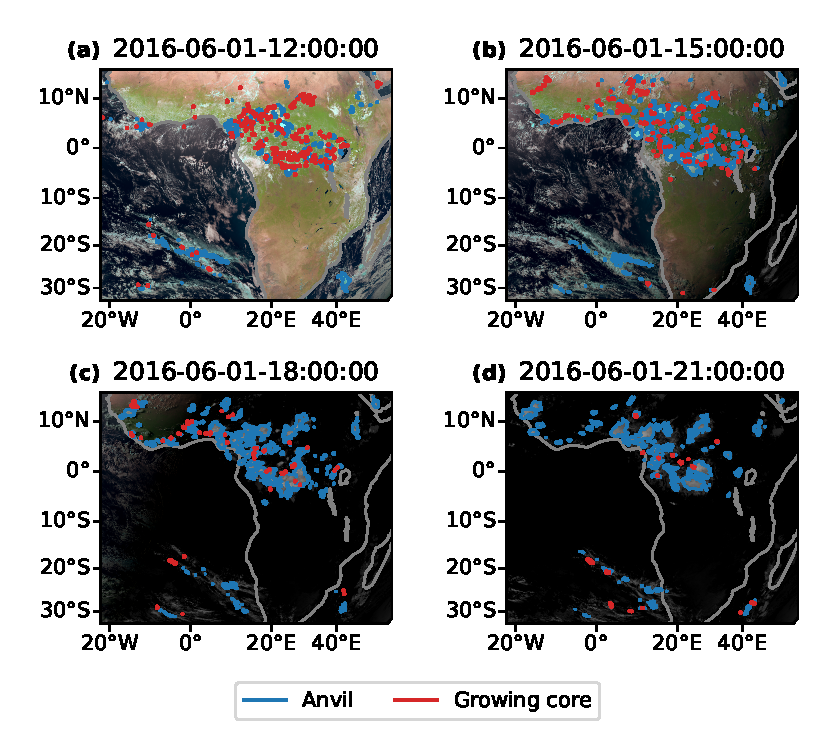
\includegraphics[width=12cm]{figures/fig04.pdf}
    \caption[
    An example of the cores and anvils (detected by tobac-flow, shown at 3-hour time intervals
    ]{
    An example of the cores (red outline) and anvils (blue outline) detected by tobac-flow plotted over visible composite imagery from \acrshort{seviri}, shown at 3-hour time intervals. All times are given in \acrshort{utc}.
    }
    \label{fig:seviri_detection}
\end{figure*}


Over the 4-month period of the case study we track a total of 145,463 cores (of which 79,592 are associated with anvil clouds) and 35,941 anvils. 
Using the detected regions of both core and anvil components of tracked \acrshort{dcc}s, the cloud properties and \acrshort{cre} are calculated for each \acrshort{dcc} at each time step from the retrieval and broadband fluxes data. 
The resulting dataset allows us to analyse the properties of each \acrshort{dcc} over their lifetimes from a Lagrangian perspective.
While the studied domain contains both land and sea regions, only a small proportion of tracked \acrshort{dcc}s occurred over sea (11\%), and so we have not separated the analysis of land and oceanic \acrshort{dcc}s in this article.

\section{Results}

\subsection{Spatial and temporal distributions}

Figure~\ref{fig:seviri_map_dists}\,a shows the frequency of core detections for each 1\texttimes 1\textdegree grid square over the period of the case study. 
The majority of observed convection occurs over the tropical rainforest regions. 
During the months of May-August, the \acrfull{itcz} is at its northernmost extent over Africa \citep{nicholson_itcz_2018}. 
The West African monsoon occurs during these months, with the primary band of convection located between 5-15\textdegree N \citep{nicholson_revised_2009}, which our observations agree with. 
We observed the maximum frequency of convection at around 6\textdegree N, 12\textdegree E over the Western High Plateau of Cameroon, with high frequencies of convection also observed over the Nigerian coastal plains to the West and the Jos Plateau in Northern Nigeria. 
High rates of convection are also observed over the coastal plains and inland highlands of Guinea, Sierra Leone and Liberia (5--12\,\textdegree N, 5--15\,\textdegree W)


\begin{figure*}[tp]
    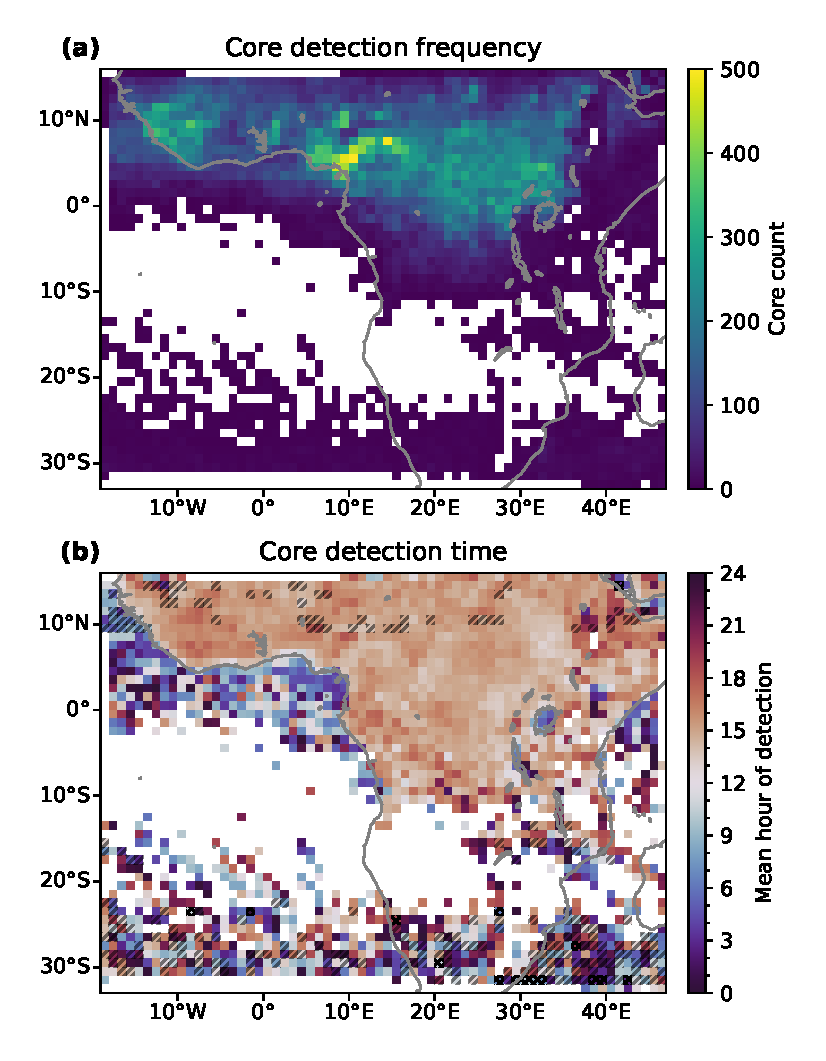
\includegraphics[width=12cm]{figures/fig05.pdf}
    \caption[
    Number of detected cores and average hour of core detection
    ]{
    a.: The total number of \acrshort{dcc} cores detected over the case study for each 1\texttimes 1\textdegree grid box. b.: The average hour of detection for the cores detected in each 1\texttimes 1\textdegree grid box. Grid boxes with a standard deviation greater than 6 hours are single-hatched, and greater than 12 hours cross-hatched.
    }
    \label{fig:seviri_map_dists}
\end{figure*}


Figure~\ref{fig:seviri_map_dists}\,b shows the average time of detection for convection in each 1\texttimes 1\textdegree grid square. 
The average is calculated as the circular mean of the local solar times of core detection in the grid square. 
Grid squares with a standard deviation greater than 6 hours (indicating a broad spread of initiation times) are given single hatching, and those with standard deviations greater than 12 hours have cross-hatching. 
The most notable feature of the time of detection is the clear contrast between land and sea. 
Convection over the land tends to occur in the afternoon (15:00--18:00), whereas over the ocean it occurs between midnight and early morning (00:00--09:00). 
Furthermore, convection over land tends to occur in a fairly narrow range of times whereas over the ocean convection occurs throughout the diurnal cycle, resulting in the hatching applied to much of the ocean region. 
There is also a noticeable lake effect on the time of convection occurring over Lake Victoria (2\textdegree S, 34\textdegree E) and Lake Tanganyika (7\textdegree S, 31\textdegree E), with convection typically observed in the early morning.

When we compare the regions of Cameroon and Nigeria (4--10\textdegree N, 6--14\textdegree E), where we detect the most cores in fig.~\ref{fig:seviri_map_dists}\,a, with the average time of detection in fig.~\ref{fig:seviri_map_dists}\,b, we see that the grid squares with more cores also tend to have an earlier average time of detection than the surrounding grid squares. 
Precipitation over the Nigerian plains and the Jos Plateau is linked to South-westerly winds bringing moist, warm air from the Gulf of Guinea \citep{vondou_seasonal_2010}. 
This warm air may then trigger convection both through the sea breeze effect and orographic lifting when it reaches the highlands, explaining both the higher frequency and earlier timing of convection compared to surrounding regions. 
A similar relationship between the high frequency of convection and earlier time of detection is also seen over the coastal region and adjacent highlands of Guinea, Sierra Leone and Liberia (5--12\textdegree N, 5--15\textdegree W) which may be due to the same mechanism.

It should be noted that due to the method of detection, cores that develop under existing anvils are less likely to be detected than those in clear sky regions. 
As a result, we may underestimate the occurrence of later occurring cores, particularly in regions such as the Northern Sahel where a second, night-time peak of precipitation has been observed.

For all further analysis, we consider only cores and anvils that are detected north of 15\textdegree S in order to constrain our analysis to tropical \acrshort{dcc}s.

\subsection{Anvil Cloud Properties}

To investigate how the behaviour of \acrshort{dcc} anvils is affected by their organisation, we group observed anvils based on how many cores are associated with them, from isolated \acrshort{dcc}s with one core to highly-clustered \acrshort{dcc}s (such as tropical cloud clusters and \acrshort{mcs}s) with 10 or more cores. 
Anvils with 6--9 cores, and with 10 or more cores, are grouped together to ensure that these groups have a comparable number of members for analysis.

Figure~\ref{fig:seviri_anvil_stats} shows properties related to the anvil area and lifetime linked to the number of cores. 
In fig.~\ref{fig:seviri_anvil_stats}\,a we show the average anvil maximum area for each group. 
We find that the maximum area increases approximately linearly with the number of cores, with increasingly clustered anvils having increasingly larger maximum areas, and highly clustered anvils having substantially larger anvils. 
Figure~\ref{fig:seviri_anvil_stats}\,b shows the average anvil lifetime compared to the number of cores. 
While the lifetime also increases with the number of cores, the difference between isolated and highly clustered anvils is proportionately smaller.


\begin{figure*}[tp]
    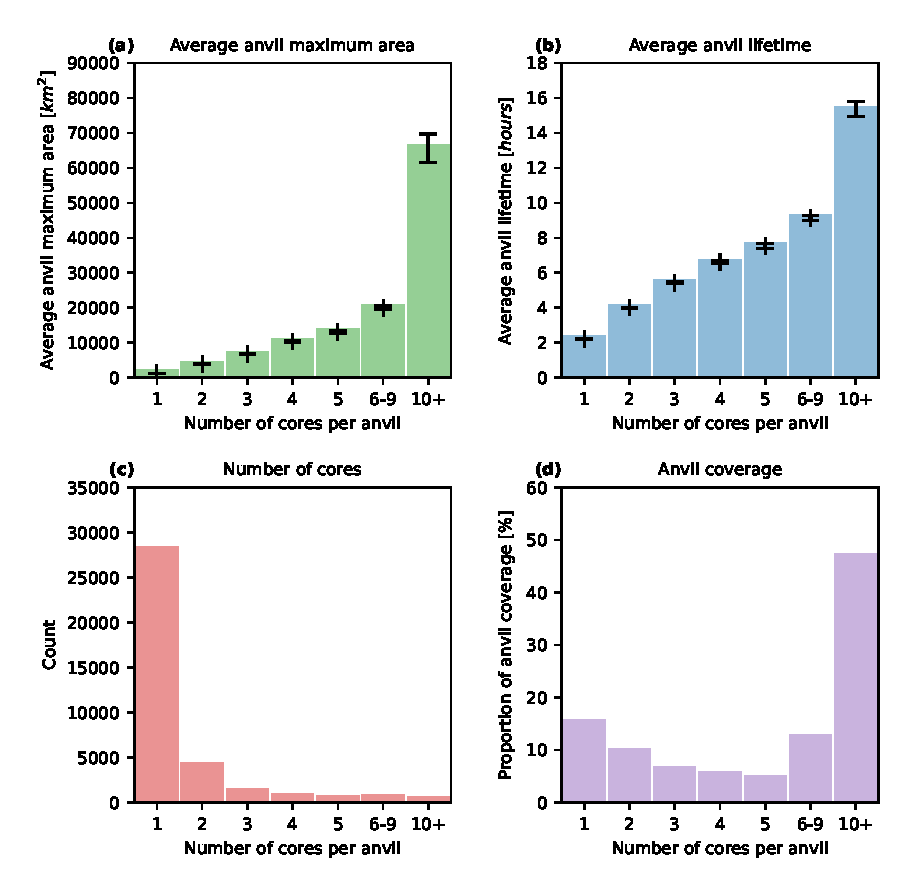
\includegraphics[width=12cm]{figures/fig06.pdf}
    \caption[
    Anvil statistics by number of associated cores for average maximum area, average lifetime, occurrence of anvils by number of cores, and percentage of total anvil coverage
    ]{
    Anvil statistics by number of associated cores for a.: average maximum area; b.: average lifetime; c.: the number of observed anvils by number of cores; and d.: percentage of total anvil coverage. Error bars in a and b show the standard error of the mean.
    }
    \label{fig:seviri_anvil_stats}
\end{figure*}


Figure~\ref{fig:seviri_anvil_stats}\,c shows the number of anvils observed with differing numbers of cores. 
We see that the vast majority of all anvils observed are isolated \acrshort{dcc}s, with over 80\% having a single detected core. 
As the number of cores increases, the number of anvils detected decreases rapidly. 
However, when considering the large increase in both anvil area and lifetime with the number of cores, the total anvil coverage for highly clustered anvils is much larger (see fig.~\ref{fig:seviri_anvil_stats}\,d). 
Despite their high frequency, isolated \acrshort{dcc}s only account for 12\% of total anvil coverage, whereas highly clustered (10+ cores) account for over 50\%. 
Previous studies have found that despite being few in number, \acrshort{mcs}s account for the majority of precipitation in Western Africa \citep{vizy_understanding_2019}.

Figure~\ref{fig:seviri_anvil_ctt_stats}\,a shows the average mean \acrshort{ctt}, and fig.~\ref{fig:seviri_anvil_ctt_stats}\,b the average minimum \acrshort{ctt} for anvils with different numbers of cores. 
While the more clustered anvils have colder average anvil \acrshort{ctt}, this decrease plateaus below 220K indicating that the reduction in clear-sky cooling below this temperature may cap the anvil \acrshort{ctt} for larger \acrshort{dcc}s. 
The minimum observed \acrshort{ctt} within each anvil, however, are colder and show a greater difference with an increasing number of cores. 
The most clustered anvils tend to have a minimum \acrshort{ctt} of around 180\,\unit{K}, indicating the presence of overshooting tops and the most intense convection. 
Care should be taken when interpreting such low retrieved \acrshort{ctt} values due to the large uncertainty associated with sensor noise at these cold temperatures.


\begin{figure*}[tp]
    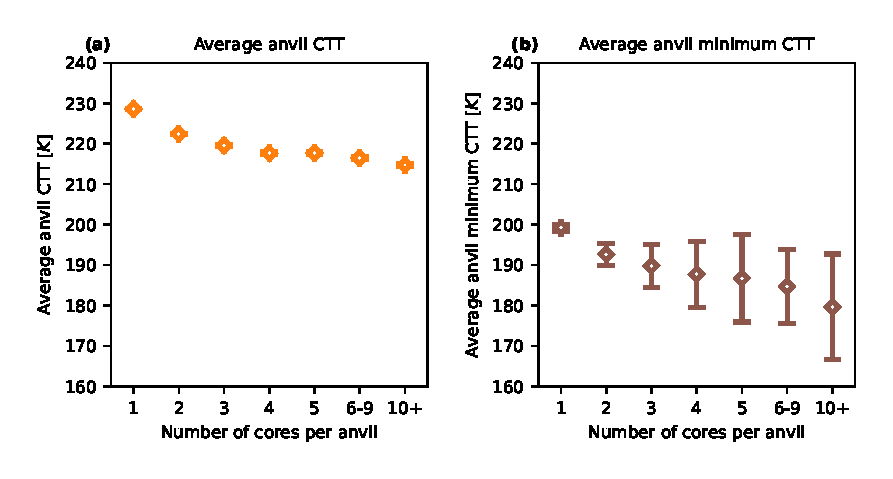
\includegraphics[width=12cm]{figures/fig07.pdf}
    \caption[
    Anvil statistics by number of cores for average anvil \acrshort{ctt} and average minimum anvil temperature
    ]{
    Anvil statistics by number of cores for a.: average anvil \acrshort{ctt}; and b.: average minimum anvil temperature. Error bars show the standard error of the mean.
    }
    \label{fig:seviri_anvil_ctt_stats}
\end{figure*}


\citet{futyan_deep_2007} divide the \acrshort{dcc} lifecycle into growing, mature and dissipating phases based on the time of observation of the coldest anvil \acrshort{ctt}, maximum anvil area and dissipation of the anvil. 
In fig.~\ref{fig:seviri_lifetime_dists} we show the distribution of the time taken to reach each of these lifecycle milestones for anvils separated by the number of associated cores. 
For all cases, the average time of minimum anvil \acrshort{ctt} occurs before the maximum area, indicating that the anvils continue to grow beyond the maximum of convective activity. 
As the number of cores associated with each anvil increases, the time of the coldest \acrshort{ctt} and largest area occur proportionately earlier during the lifetime of the anvil. 
As a result, these more clustered anvils spend more of their lifetime existing with warming, shrinking anvils than the isolated \acrshort{dcc}s.


\begin{figure*}[tp]
    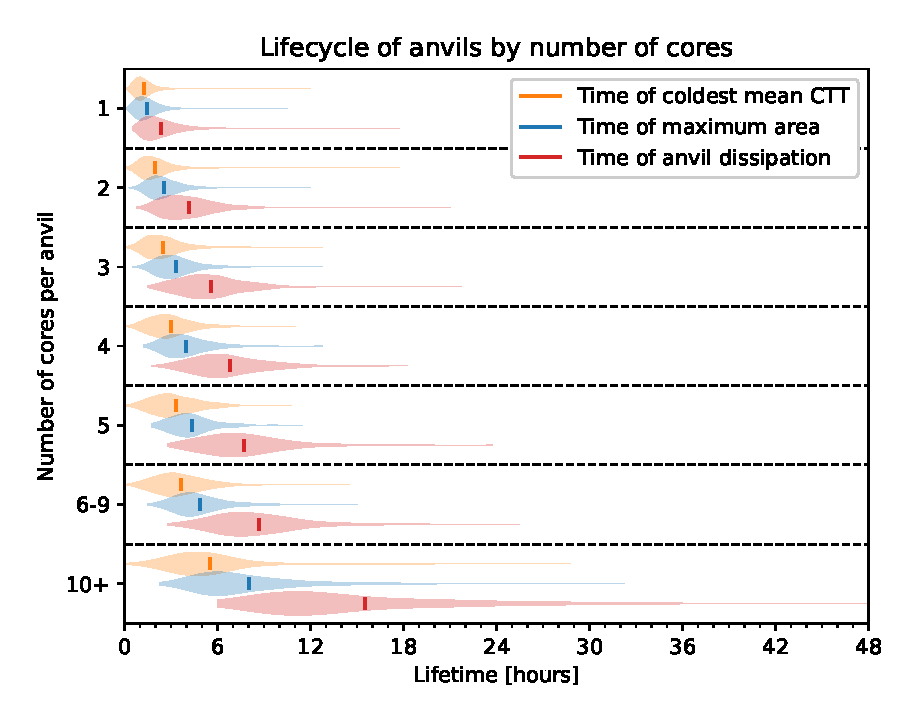
\includegraphics[width=12cm]{figures/fig08.pdf}
    \caption[
    The distribution of time to coldest mean anvil \acrshort{ctt}, largest anvil area and time of anvil dissipation
    ]{
    The distribution of time to coldest mean anvil \acrshort{ctt} (orange), largest anvil area (green) and time of anvil dissipation (red) for anvils grouped by number of cores. The vertical lines show the mean time for each distribution.
    }
    \label{fig:seviri_lifetime_dists}
\end{figure*}


In fig.~\ref{fig:seviri_lifetime_proportions}, we compare the proportion of the overall anvil lifetime spent in each of the lifecycle phases defined by \citet{futyan_deep_2007} to the number of cores associated with the anvil. 
There is a clear trend that, as the number of cores increases, the proportion of the lifecycle spent in the growing phase decreases, and the proportion spent in the mature and dissipating phases increases.
 Although this approach to classifying the lifecycle of anvil clouds is simplistic and does not capture the complexities of large, long-lived \acrshort{dcc}s which may go through multiple cycles of growth, dissipation and re-invigoration, it can provide a useful perspective when considering the \acrshort{lw} \acrshort{cre} of \acrshort{dcc}s. 
 The time of the coldest average \acrshort{ctt} will be when the \acrshort{lw} \acrshort{cre} of the anvil cloud is at its greatest, and so can help understand the evolution of the anvil \acrshort{cre} over its lifetime.


\begin{figure*}[tp]
    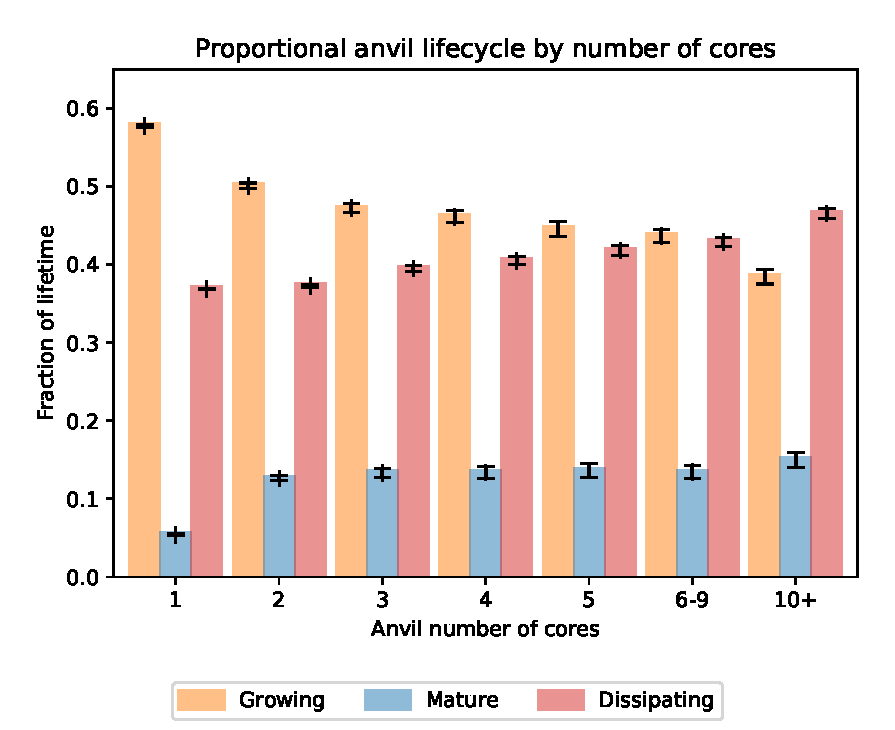
\includegraphics[width=12cm]{figures/fig09.pdf}
    \caption[
    The proportion of anvil lifetime spent in the growing, mature and dissipating phase
    ]{
    The proportion of anvil lifetime spent in the growing (orange), mature (green) and dissipating (red) phase, according to the criteria used by \citet{futyan_deep_2007}
    }
    \label{fig:seviri_lifetime_proportions}
\end{figure*}


\subsection{Anvil \acrshort{cre}}

Using the broadband fluxes data in conjunction with the tracked \acrshort{dcc} dataset, we are able to track how the \acrshort{sw}, \acrshort{lw} and net \acrshort{cre} evolve over the lifetime of each tracked anvil.
Figure~\ref{fig:cre_lifecycle_examples} shows the time series of \acrshort{sw}, \acrshort{lw} and net \acrshort{cre} as well as the cumulative average \acrshort{cre} (the average of net \acrshort{cre} over anvil area and lifetime up until that point in time) for several different anvil lifecycles.
Note that all fluxes are \acrshort{toa} and measured in the downward direction, so a positive value represents warming and a negative value represents cooling.


\begin{figure*}[tp]
    \centering
    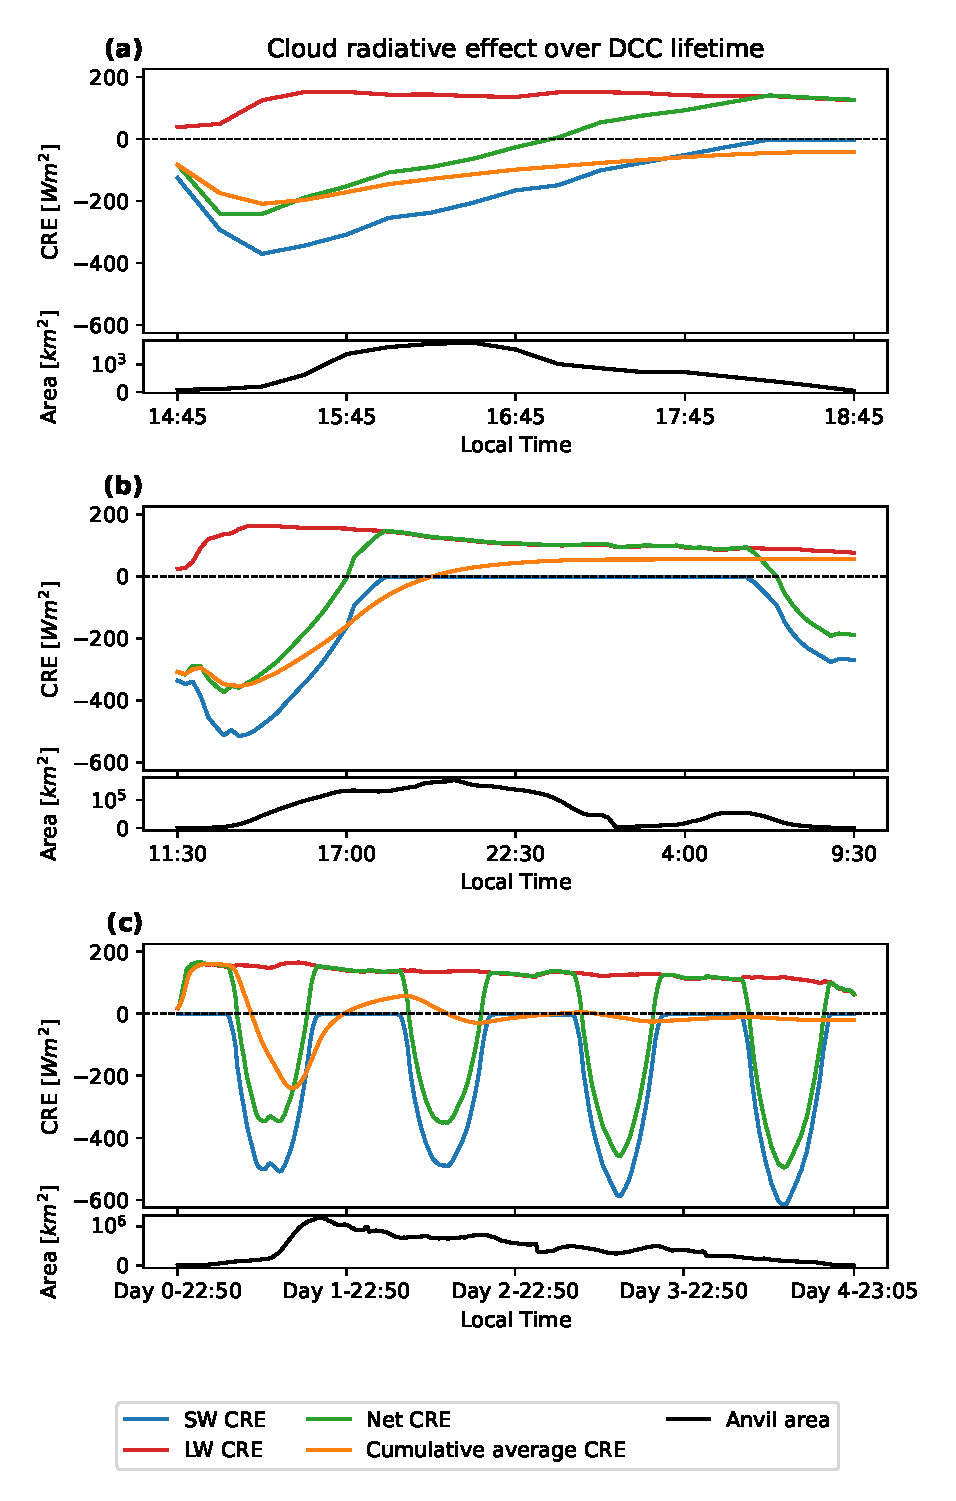
\includegraphics[width=10.8cm]{figures/fig10.pdf}
    \caption[
    Anvil net, \acrshort{lw}, and \acrshort{sw} \acrshort{cre}, cumulative mean \acrshort{cre} over anvil lifetime
    ]{
    Anvil net, \acrshort{lw}, and \acrshort{sw} \acrshort{cre}, cumulative mean \acrshort{cre} over anvil lifetime and anvil area for a.: an isolated, short-lived (4-hour) \acrshort{dcc}; b.: a moderately clustered, 1-day long \acrshort{dcc}; and c.: a large, clustered, 4-day long \acrshort{dcc}. All times are the local solar time, to the nearest 5-minute interval. The black lines show the change in area of each \acrshort{dcc} over their lifecycle.
    }
    \label{fig:cre_lifecycle_examples}
\end{figure*}


Figure~\ref{fig:cre_lifecycle_examples}\,a shows the case of an isolated, short-lived \acrshort{dcc}. 
The \acrshort{dcc} initiates during the daytime, during which the \acrshort{sw} \acrshort{cre} dominates and the net \acrshort{cre} is negative (cooling). 
However, towards the end of the four-hour lifecycle of the \acrshort{dcc}, it transitions to night-time and so while the \acrshort{sw} \acrshort{cre} reduces and eventually becomes zero, the \acrshort{lw} \acrshort{cre} dominates and the net \acrshort{cre} is positive (warming). 
While this period of warming moves the cumulative average \acrshort{cre} towards zero, it remains overall negative for the overall lifetime of the \acrshort{dcc} both due to the longer period spent during the daytime, and the larger area of the anvil cloud during this period.

Figure~\ref{fig:cre_lifecycle_examples}\,b shows the case of a longer-lived (22 hours), clustered \acrshort{dcc}. 
It initiates in the morning, and so the \acrshort{sw} cooling dominates for the first half of the anvil lifetime. 
Compared to the isolated \acrshort{dcc}, it exists for much longer during the night time, and so the cumulative average becomes positive over the full lifetime of the anvil cloud.

Figure~\ref{fig:cre_lifecycle_examples}\,c shows the case of a four-day, highly clustered convective event. 
In this case, we see the net \acrshort{cre} alternates between warming and cooling throughout the diurnal cycle. 
The cumulative \acrshort{cre} also alternates between overall warming and cooling throughout the lifetime of the anvil and results in a small net cooling effect.

We see in both the longer-lived cases (fig.~\ref{fig:cre_lifecycle_examples}\,b, c) that the \acrshort{lw} \acrshort{cre} reduces towards the end of the anvil cloud lifetime. 
This may be reflective of the findings from fig.~\ref{fig:seviri_lifetime_dists} that the minimum average \acrshort{ctt} occurs before the mid-point of the cloud lifecycle for longer-lived systems. 
This reduction in \acrshort{lw} \acrshort{cre} may be due to a thinning of the anvil cloud (allowing increased \acrshort{lw} emission from the surface), or due to heating and stabilisation of the upper troposphere by the \acrshort{dcc}.
In addition, the cumulative radiative cooling of the anvil top may drive subsidence and reduce the cloud-top height of the anvil over time \citep{sokol_tropical_2020}

Figure~\ref{fig:anvil_cre_dist} shows the distribution of net lifetime \acrshort{cre} for all tracked anvils. 
The overall negative average value of --\,0.94\,\textpm\,0.91\,\unit{W m^{-2}} is very close to zero considering the large spread in \acrshort{cre}. 
However, the distribution shows a bimodal structure, with two peaks at around +\,100\,\unit{W m^{-2}} (warming) and --\,180\,\unit{W m^{-2}} (cooling). 
The distribution is coloured according to the mean number of cores associated with the anvils in each bin of the distribution. 
Both the peaks of the distribution are mainly composed of isolated \acrshort{dcc}s which occur during the daytime (negative peak) or night-time (positive peak). 
The centre of the distribution---with average \acrshort{cre}s close to zero---shows a greater number of the clustered \acrshort{dcc}s with multiple cores which, due to their longer lifetime, tend to exist during both the day- and night time.


\begin{figure*}[tp]
    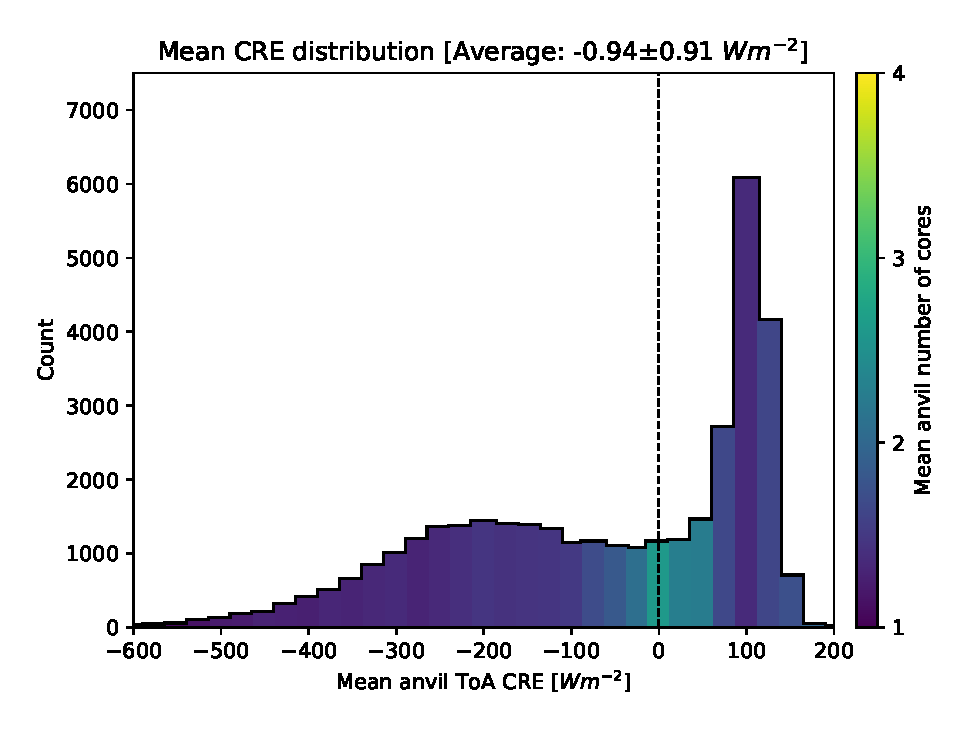
\includegraphics[width=12cm]{figures/fig11.pdf}
    \caption[
    The distribution of lifetime anvil \acrshort{cre} for all observed anvils
    ]{
    The distribution of lifetime anvil \acrshort{cre} for all observed anvils. The mean number of cores per anvil in each bin is indicated by the colour scale. The vertical dashed line shows the integrated mean \acrshort{cre} (over area and lifetime) over all anvils, weighted by the anvil areas (--0.94\,\textpm\,0.91\,\unit{W m^{-2}}).
    }
    \label{fig:anvil_cre_dist}
\end{figure*}


In fig.~\ref{fig:anvil_sw_lw_cre} we break down the \acrshort{cre} distribution into that of the \acrshort{sw} (fig.~\ref{fig:anvil_sw_lw_cre}\,a) and \acrshort{lw} (fig.~\ref{fig:anvil_sw_lw_cre}\,b) components. 
The \acrshort{sw} \acrshort{cre} shows a similar bimodal distribution to that of the net \acrshort{cre}, whereas the \acrshort{lw} distribution shows a normal distribution. 
The \acrshort{sw} \acrshort{cre} has a large peak at 0\,\unit{W m^{-2}} for \acrshort{dcc}s that occur during the night-time, and a broad peak centred around --\,300\,\unit{W m^{-2}} consisting of daytime \acrshort{dcc}s, with the average falling between the two. 
Note that the average for the \acrshort{lw} falls to the right of the peak of the distribution because the average is integrated over the anvil area and lifetime, and the largest and longest-lived anvils tend to have colder \acrshort{ctt} and hence larger \acrshort{lw} \acrshort{cre}.


\begin{figure*}[tp]
    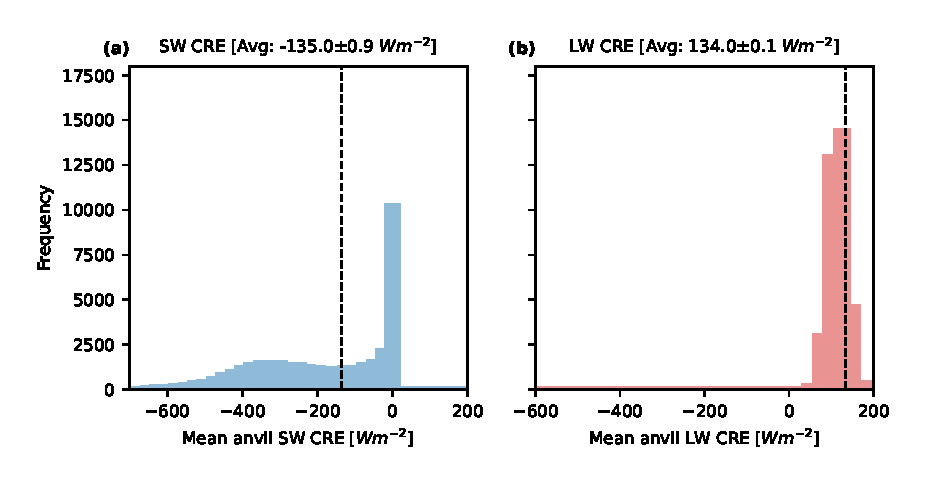
\includegraphics[width=12cm]{figures/fig12.pdf}
    \caption[
    The distributions of mean anvil \acrshort{sw} \acrshort{cre} and \acrshort{lw} \acrshort{cre}
    ]{
    The distributions of mean anvil \acrshort{sw} \acrshort{cre} (a) and \acrshort{lw} \acrshort{cre} (b). The vertical dashed line shows the integrated mean \acrshort{cre} over all anvils (\acrshort{sw}: -135.0\,\textpm\,0.9\,\unit{W m^{-2}}, \acrshort{lw}: 134.0\,\textpm\,0.1\,\unit{W m^{-2}})
    }
    \label{fig:anvil_sw_lw_cre}
\end{figure*}


Figure~\ref{fig:anvil_cre_time_vs_ctt} shows (a) the average instantaneous anvil \acrshort{cre} binned by the time of observation (local solar time) and mean anvil \acrshort{ctt}, and (b) the average lifetime anvil \acrshort{cre} binned by time of initial detection (local solar time) and mean anvil \acrshort{ctt}.
We see that, as expected, mean anvil \acrshort{cre} becomes more positive with decreasing \acrshort{ctt} due to increased \acrshort{lw} warming. 
However, the diurnal cycle of detection shows a much stronger contrast, with anvils detected during the daytime having a net cooling effect compared to those at night which have a net warming \acrshort{cre}. 
This diurnal cycle effect is stronger for those anvils with warmer average \acrshort{ctt}, generally representing isolated, shorter-lived \acrshort{dcc}s, and is weaker for colder anvil \acrshort{ctt}. 
Note also that in fig.~\ref{fig:seviri_anvil_ctt_stats}\,b that the phase of the diurnal cycle shifts to earlier times of detection as average anvil \acrshort{ctt} become colder, as these \acrshort{dcc}s tend to have longer lifetimes.


\begin{figure*}[tp]
    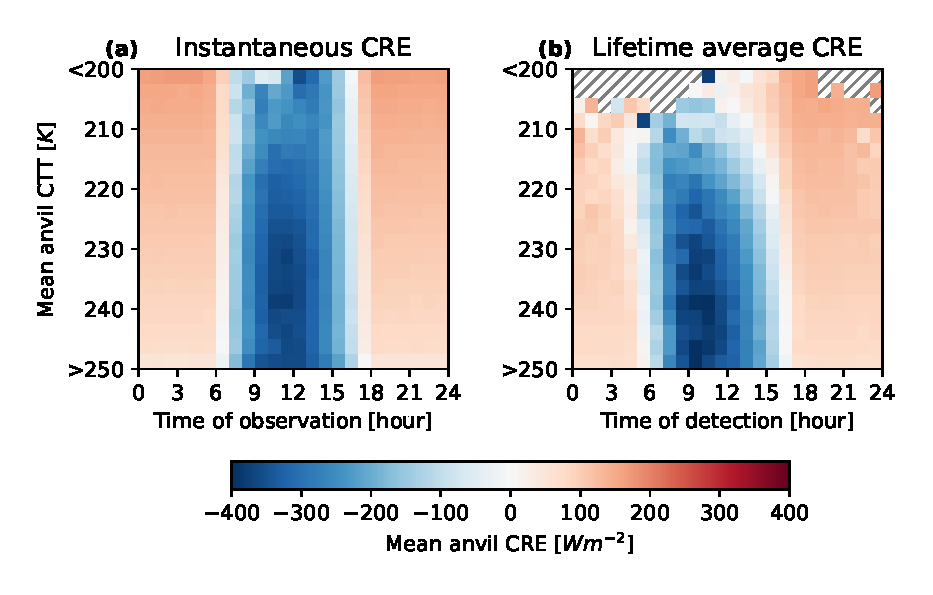
\includegraphics[width=12cm]{figures/fig13.pdf}
    \caption[
    Average anvil \acrshort{cre} binned by the time of detection (local time) and mean anvil \acrshort{ctt}
    ]{
    (a) Average instantaneous anvil \acrshort{cre} binned by the time of observation (local solar time) and mean anvil \acrshort{ctt}. (b) Average lifetime anvil \acrshort{cre} binned by time of initial detection (local solar time) and mean anvil \acrshort{ctt}. Hashed regions in (b) show bins in which no anvils were detected.
    }
    \label{fig:anvil_cre_time_vs_ctt}
\end{figure*}


It is apparent from figs.~\ref{fig:anvil_cre_dist} and \ref{fig:anvil_sw_lw_cre} that the observed neutral net anvil \acrshort{cre} is not only due to a balance between the \acrshort{sw} and \acrshort{lw}, but also from a balance of the cooling effect of daytime \acrshort{dcc}s and the warming effect of those occurring at night. 
If the number of \acrshort{dcc}s occurring during the daytime were to reduce we would expect a net warming effect without any change to the \acrshort{cre} of individual \acrshort{dcc}s.
As the diurnal cycle of convection over the ocean is nearly uniform, we should expect little impact on anvil \acrshort{cre} from changes in the time of convective initiation.
However, over land, where convective activity is much more common in the afternoon, changes in the diurnal cycle may have a much larger effect on anvil \acrshort{cre}.

Furthermore, fig.~\ref{fig:anvil_cre_time_vs_ctt}\,b highlights that differences in anvil temperature are linked to the diurnal cycle of anvil \acrshort{cre} as colder anvils tend to have longer lifetimes.
As a result, if warming surface temperatures lead to the invigoration of \acrshort{dcc}s, the warming effect we would see would be larger than the \acrshort{lw} effect from the change in anvil temperature alone. 
Surface warming may also result in an earlier time of convective initiation, resulting in a cooling feedback.


\conclusions  %% \conclusions[modified heading if necessary]

By combining a novel cloud tracking algorithm with a new dataset of derived all-sky and clear-sky fluxes from geostationary satellite observations, we were able to detect and track \acrshort{dcc} anvils and their associated cores for both isolated and clustered \acrshort{dcc}s and investigate their properties, lifecycle and \acrshort{cre}. 
As this study was performed using data from May-August (Northern hemisphere summer), we observed the majority of convective activity over the Guinea-Congo rainforest and Savanna regions, as the \acrshort{itcz} is at its northernmost extent.

We evaluate the degree of convective clustering of each anvil by measuring the number of cores it is associated with. 
We find that, as expected, anvils with the greatest number of cores---including \acrshort{mcs}s---have larger anvil areas, longer lifetimes and the coldest cloud tops. 
As a result, despite the majority of observed \acrshort{dcc}s being isolated, the highly clustered anvils make up most of the anvil coverage, and so cause most of the anvil impact over this region. 
We also find that the proportion of the lifecycle spent in the mature and dissipating phases increases with the number of cores, and the proportion spent in the growing phase decreases.

When looking into the net \acrshort{cre} of anvils, we find that, although the average \acrshort{cre} across all observed anvils is close to zero, few anvils have near zero \acrshort{cre} themselves. 
We find a bimodal distribution of anvil \acrshort{cre}, with isolated \acrshort{dcc}s that exist during the daytime causing the negative (cooling) peak, and those that exist during the night-time causing the positive (warming) peak. 
The systems with near zero \acrshort{cre} tend to live longer with more cores, and exist during both the day- and night-time. 
As a result, when considering the magnitude of the anvil \acrshort{cre}, isolated \acrshort{dcc}s have an outsized contribution to the overall average anvil \acrshort{cre} of 21.4\% compared to their proportion of all anvil coverage (15.3\%) (see supplementary fig. S4).

The interaction between the diurnal cycle of convection and \acrshort{dcc} lifetime plays a key role in the shape of the \acrshort{sw} anvil \acrshort{cre} distribution and is important to consider in regard to anvil \acrshort{cre} feedback. 
As the \acrshort{lw} \acrshort{cre} is normally distributed, a response to changing cloud top height or temperature may occur as a shift in the distribution. 
However, the bimodal distribution of the \acrshort{sw} \acrshort{cre} must result in more complex adjustments to shift the overall mean. 
As the position of the peak at 0 \,\unit{W m^{-2}} relating to night-time \acrshort{dcc}s is fixed, to change the overall average \acrshort{sw} \acrshort{cre} either the width of the distribution has to increase or decrease, or the number of \acrshort{dcc}s occurring during the day- or night-time has to increase. 
The former has important implications for the diurnal cycle of temperature in the tropics, and the latter for the diurnal cycle of convection, which, in turn, affects the anvil lifecycle.

Changes in the diurnal cycle of convection may not have a large impact on net anvil \acrshort{cre} over the ocean due to the mostly uniform occurrence of convection throughout the day.
Over land, however, the afternoon peak of convection at around 3\,pm solar time (see fig.~\ref{fig:seviri_map_dists}) coincides with a time at which anvil \acrshort{cre} is very sensitive to shifts in the diurnal cycle (fig.~\ref{fig:anvil_cre_time_vs_ctt}\,b).
Furthermore, a reduction or increase in the number of \acrshort{dcc}s occurring at a specific time of day may change the net \acrshort{cre} of anvils without any change in the \acrshort{cre} of individual \acrshort{dcc}s.

Diagnosing a diurnal cycle related anvil cloud feedback in climate models may however be difficult.
While \citet{beydoun_dissecting_2021} found that changes in anvil lifetime contributed little to \acrshort{cre} feedbacks, this study used a radiative-convective-equilibrium model with no diurnal cycle of insolation.
Although convective-resolving models have been found to model the diurnal cycle an lifecycle of \acrshort{dcc}s better than parameterised climate models \citep{prein_review_2015, feng_mesoscale_2023}, but lack good observational constraints.
Disentangling the impacts of convective processes and anvil cirrus processes on anvil lifecycle and \acrshort{cre} is also a key challenge.
Here, the use of model experiments such as that of \citet{gasparini_diurnal_2022} may help better understand the impacts of both processes on anvil \acrshort{cre} and the potential for climate feedbacks.

There are, however, a number of limitations in this study which present opportunities for future research. 
Firstly, as this study only involved 4 months of data during the Northern Hemisphere summer, we were not able to investigate the impact of the seasonal cycle on the behaviour of \acrshort{dcc}s and their \acrshort{cre}. 
Furthermore, extending to a larger domain would allow investigation of regional differences, in particular the important land--sea contrast of deep convection \citep{takahashi_revisiting_2023}. 
A major limitation of the \acrshort{seviri} data is its poor sensitivity to thin anvil cirrus, which has an important impact on net anvil \acrshort{cre} \citep{protopapadaki_upper_2017, horner_evolution_2023}.
The flexible combined imager \citep{martin_fci_2021} aboard the third-generation Meteosat may allow better detection and study of thin anvil cirrus over tropical Africa in the near future.

Cloud tracking provides a key capability for the study of deep convective anvil clouds \citep{gasparini_opinion_2023b}.
The ability to observe changes over the lifetime of an anvil cloud independently of changes in the microphysical or macrophysical properties of \acrshort{dcc}s.
Further application of cloud tracking approaches may better our understanding of \acrshort{dcc} lifecycle, its relation to the diurnal cycle of radiation, and its response to a changing climate.



%% The following commands are for the statements about the availability of data sets and/or software code corresponding to the manuscript.
%% It is strongly recommended to make use of these sections in case data sets and/or software code have been part of your research the article is based on.

% \codeavailability{TEXT} %% use this section when having only software code available


% \dataavailability{TEXT} %% use this section when having only data sets available


\codedataavailability{
The CC4CL cloud retrieval algorithm is available for use with the GPL v3.0 licence and can be accessed through the following github repository: \url{https://github.com/ORAC-CC/orac}.
The tobac-flow DCC detection and tracking algorithm is available under the BSD 3-clause licence.
Version 1.7.6, which was utilised for this study, is archived at the following repository: \url{https://zenodo.org/record/8317062} \citep{jones_tobacflow_2023}.
Radiative transfer simulations were performed using libRadtran \citep{emde_libradtran_2016}.
We thank EUMETSAT for the provision of the Meteosat SEVIRI level 1.5 data used in this study, which is openly available via the EUMETSAT data store.
CERES EBAF edition 4.2 used for calibration were obtained from the NASA Langley Research Center Atmospheric Sciences Data Center.

The dataset of tracked DCCs and their properties used in this study is available at the following repository: \url{https://zenodo.org/records/8317025} \citep{jones_cloudcci_2023}.
The material used to prepare this manuscript, including code used to perform analysis and preparation of figures, is archived at the following repository: \url{https://zenodo.org/records/10696901} \citep{jones_material_2024}.
} %% use this section when having data sets and software code available


% \sampleavailability{TEXT} %% use this section when having geoscientific samples available


% \videosupplement{TEXT} %% use this section when having video supplements available


% \appendix
% \section{}    %% Appendix A

% \subsection{}     %% Appendix A1, A2, etc.


\noappendix       %% use this to mark the end of the appendix section. Otherwise the figures might be numbered incorrectly (e.g. 10 instead of 1).

%% Regarding figures and tables in appendices, the following two options are possible depending on your general handling of figures and tables in the manuscript environment:

%% Option 1: If you sorted all figures and tables into the sections of the text, please also sort the appendix figures and appendix tables into the respective appendix sections.
%% They will be correctly named automatically.

%% Option 2: If you put all figures after the reference list, please insert appendix tables and figures after the normal tables and figures.
%% To rename them correctly to A1, A2, etc., please add the following commands in front of them:

% \appendixfigures  %% needs to be added in front of appendix figures

% \appendixtables   %% needs to be added in front of appendix tables

%% Please add \clearpage between each table and/or figure. Further guidelines on figures and tables can be found below.



\authorcontribution{WKJ designed the study. MS produced the dataset of retrieved cloud properties and radiative fluxes. WKJ performed the detection and tracking and the data analysis. WKJ wrote this article with contributions from MS and PS.} %% this section is mandatory

\competinginterests{At least one of the (co-)authors is a member of the editorial board of Atmospheric Chemistry and Physics.} %% this section is mandatory even if you declare that no competing interests are present

% \disclaimer{TEXT} %% optional section

\begin{acknowledgements}
The authors acknowledge financial support from the European Research Council (ERC), H2020 European Research Council RECAP (grant no.724602), and from the European Space Agency (ESA) through the Cloud\_cci project (contract no.: 4000128637/20/INB). Philip Stier additionally acknowledges funding from the FORCeS and NextGEMs projects under the European Union's Horizon 2020 research program with Grants 821205 and 101003470, respectively. We thank EUMETSAT for providing the Meteosat-11 SEVIRI data used in this study. The processing of retrieved cloud properties and derived broadband fluxes was performed at DWD. The production and analysis of the tracked DCCs dataset were performed on JASMIN: the UK collaborative data analysis facility; and LOTUS: the associated high-performance batch compute cluster.

\end{acknowledgements}




%% REFERENCES

%% The reference list is compiled as follows:

% \begin{thebibliography}{}

% \bibitem[AUTHOR(YEAR)]{LABEL1}
% REFERENCE 1

% \bibitem[AUTHOR(YEAR)]{LABEL2}
% REFERENCE 2

% \end{thebibliography}

%% Since the Copernicus LaTeX package includes the BibTeX style file copernicus.bst,
%% authors experienced with BibTeX only have to include the following two lines:
%%
\bibliographystyle{copernicus}
\bibliography{bibliography.bib}
%%
%% URLs and DOIs can be entered in your BibTeX file as:
%%
%% URL = {http://www.xyz.org/~jones/idx_g.htm}
%% DOI = {10.5194/xyz}


%% LITERATURE CITATIONS
%%
%% command                        & example result
%% \citet{jones90}|               & Jones et al. (1990)
%% \citep{jones90}|               & (Jones et al., 1990)
%% \citep{jones90,jones93}|       & (Jones et al., 1990, 1993)
%% \citep[p.~32]{jones90}|        & (Jones et al., 1990, p.~32)
%% \citep[e.g.,][]{jones90}|      & (e.g., Jones et al., 1990)
%% \citep[e.g.,][p.~32]{jones90}| & (e.g., Jones et al., 1990, p.~32)
%% \citeauthor{jones90}|          & Jones et al.
%% \citeyear{jones90}|            & 1990



%% FIGURES

%% When figures and tables are placed at the end of the MS (article in one-column style), please add \clearpage
%% between bibliography and first table and/or figure as well as between each table and/or figure.

% The figure files should be labelled correctly with Arabic numerals (e.g. fig01.jpg, fig02.png).


%% ONE-COLUMN FIGURES

%%f
%\begin{figure}[t]
%\includegraphics[width=8.3cm]{FILE NAME}
%\caption{TEXT}
%\end{figure}
%
%%% TWO-COLUMN FIGURES
%
%%f
%\begin{figure*}[t]
%\includegraphics[width=12cm]{FILE NAME}
%\caption{TEXT}
%\end{figure*}
%
%
%%% TABLES
%%%
%%% The different columns must be seperated with a & command and should
%%% end with \\ to identify the column brake.
%
%%% ONE-COLUMN TABLE
%
%%t
%\begin{table}[t]
%\caption{TEXT}
%\begin{tabular}{column = lcr}
%\tophline
%
%\middlehline
%
%\bottomhline
%\end{tabular}
%\belowtable{} % Table Footnotes
%\end{table}
%
%%% TWO-COLUMN TABLE
%
%%t
%\begin{table*}[t]
%\caption{TEXT}
%\begin{tabular}{column = lcr}
%\tophline
%
%\middlehline
%
%\bottomhline
%\end{tabular}
%\belowtable{} % Table Footnotes
%\end{table*}
%
%%% LANDSCAPE TABLE
%
%%t
%\begin{sidewaystable*}[t]
%\caption{TEXT}
%\begin{tabular}{column = lcr}
%\tophline
%
%\middlehline
%
%\bottomhline
%\end{tabular}
%\belowtable{} % Table Footnotes
%\end{sidewaystable*}
%
%
%%% MATHEMATICAL EXPRESSIONS
%
%%% All papers typeset by Copernicus Publications follow the math typesetting regulations
%%% given by the IUPAC Green Book (IUPAC: Quantities, Units and Symbols in Physical Chemistry,
%%% 2nd Edn., Blackwell Science, available at: http://old.iupac.org/publications/books/gbook/green_book_2ed.pdf, 1993).
%%%
%%% Physical quantities/variables are typeset in italic font (t for time, T for Temperature)
%%% Indices which are not defined are typeset in italic font (x, y, z, a, b, c)
%%% Items/objects which are defined are typeset in roman font (Car A, Car B)
%%% Descriptions/specifications which are defined by itself are typeset in roman font (abs, rel, ref, tot, net, ice)
%%% Abbreviations from 2 letters are typeset in roman font (RH, LAI)
%%% Vectors are identified in bold italic font using \vec{x}
%%% Matrices are identified in bold roman font
%%% Multiplication signs are typeset using the LaTeX commands \times (for vector products, grids, and exponential notations) or \cdot
%%% The character * should not be applied as mutliplication sign
%
%
%%% EQUATIONS
%
%%% Single-row equation
%
%\begin{equation}
%
%\end{equation}
%
%%% Multiline equation
%
%\begin{align}
%& 3 + 5 = 8\\
%& 3 + 5 = 8\\
%& 3 + 5 = 8
%\end{align}
%
%
%%% MATRICES
%
%\begin{matrix}
%x & y & z\\
%x & y & z\\
%x & y & z\\
%\end{matrix}
%
%
%%% ALGORITHM
%
%\begin{algorithm}
%\caption{...}
%\label{a1}
%\begin{algorithmic}
%...
%\end{algorithmic}
%\end{algorithm}
%
%
%%% CHEMICAL FORMULAS AND REACTIONS
%
%%% For formulas embedded in the text, please use \chem{}
%
%%% The reaction environment creates labels including the letter R, i.e. (R1), (R2), etc.
%
%\begin{reaction}
%%% \rightarrow should be used for normal (one-way) chemical reactions
%%% \rightleftharpoons should be used for equilibria
%%% \leftrightarrow should be used for resonance structures
%\end{reaction}
%
%
%%% PHYSICAL UNITS
%%%
%%% Please use \unit{} and apply the exponential notation


\end{document}
